% Created 2012-11-29 Thu 15:42
\documentclass[serif,11pt]{beamer}
\usepackage[utf8]{inputenc}
\usepackage[T1]{fontenc}
\usepackage{fixltx2e}
\usepackage{graphicx}
\usepackage{longtable}
\usepackage{float}
\usepackage{wrapfig}
\usepackage{soul}
\usepackage{textcomp}
\usepackage{marvosym}
\usepackage{wasysym}
\usepackage{latexsym}
\usepackage{amssymb}
\usepackage{hyperref}
\tolerance=1000
\usepackage{fourier}
\usepackage{amsmath}
\newcommand{\R}{\textsuperscript{\textregistered}}
\providecommand{\alert}[1]{\textbf{#1}}

\title{Highly Accurate Consensus Sequence and Genome Assembly using PacBio\R  \emph{RS} Sequence Data}
\author{David H. Alexander, Ph.D. \newline  Pacific Biosciences}
\date{\today}
\hypersetup{
  pdfkeywords={},
  pdfsubject={},
  pdfcreator={Emacs Org-mode version 7.8.11}}

\begin{document}

\maketitle


\section{Outline}
\label{sec-1}
\begin{frame}
\frametitle{Outline}
\label{sec-1-1}

\begin{itemize}
\item History of DNA sequencing
\item PacBio SMRT\R sequencing in a nutshell
\item A genome assembly primer
\item HGAP assembly procedure
\item High accuracy consensus: the Quiver algorithm
\end{itemize}
\end{frame}
\section{History of DNA sequencing}
\label{sec-2}
\begin{frame}

   \sectionpage
\end{frame}
\begin{frame}
\frametitle{Generation 1: Sanger sequencing}
\label{sec-2-1}

   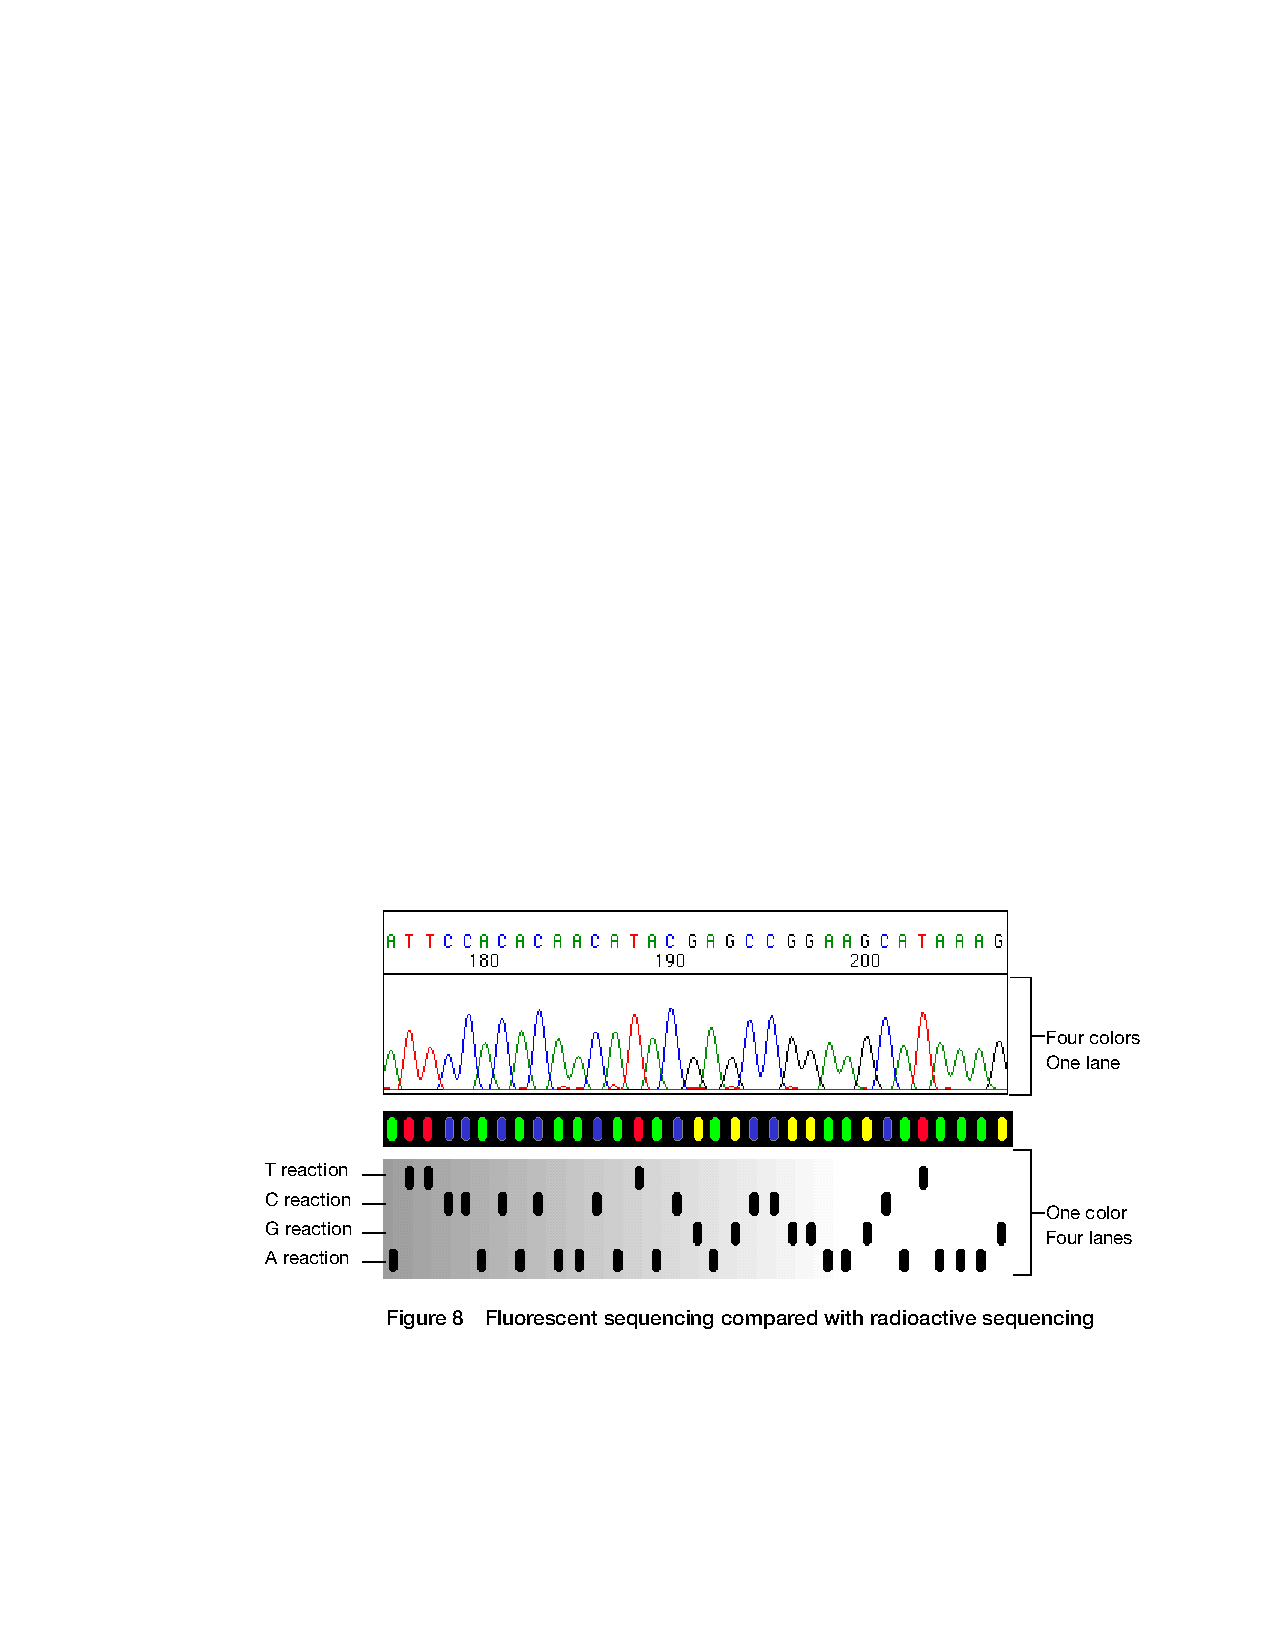
\includegraphics[width=4.5in]{img/capillary-sanger.pdf}

\begin{itemize}
\item Dideoxy chain termination
\item Longish reads ($\sim700$ bp). High accuracy. Low throughput
\end{itemize}
\end{frame}
\begin{frame}
\frametitle{Generation 2: High-throughput short-read technologies}
\label{sec-2-2}

   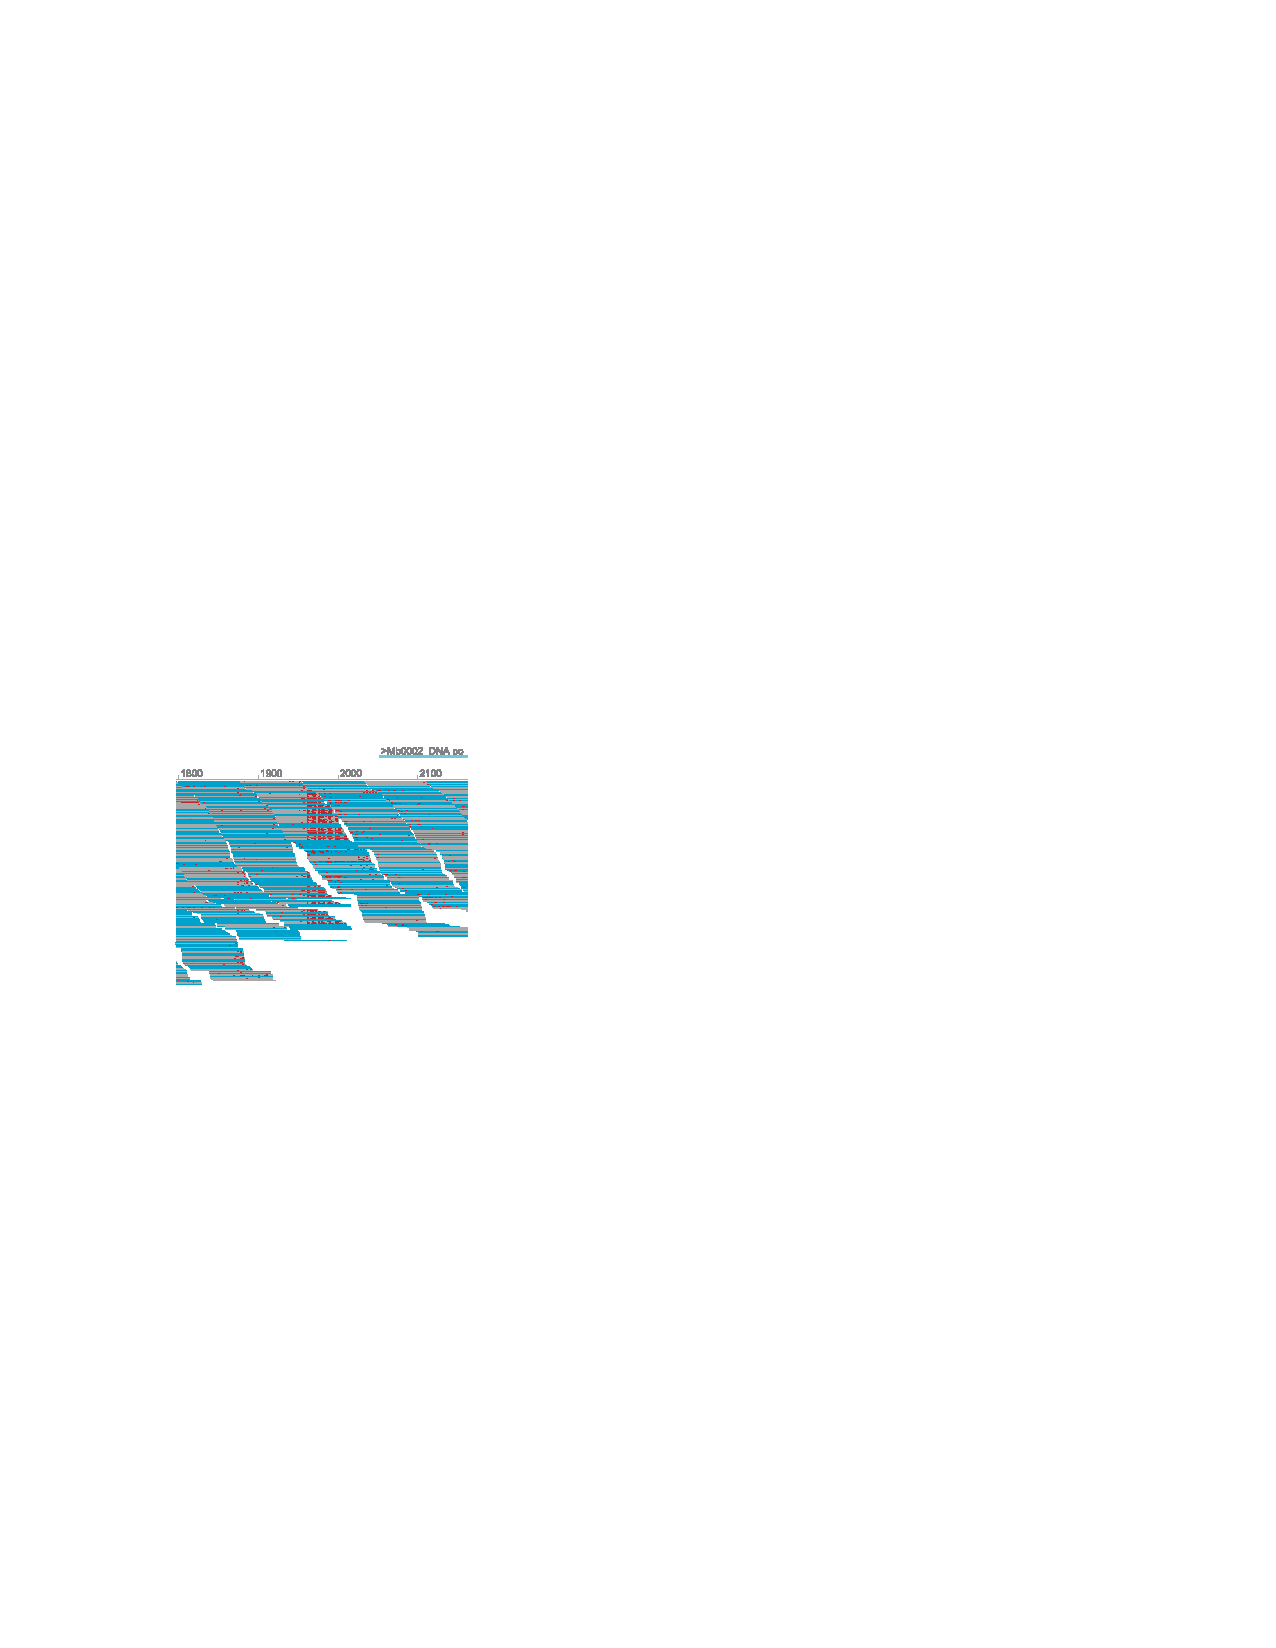
\includegraphics[width=2in]{img/short-reads-pileup.pdf}
   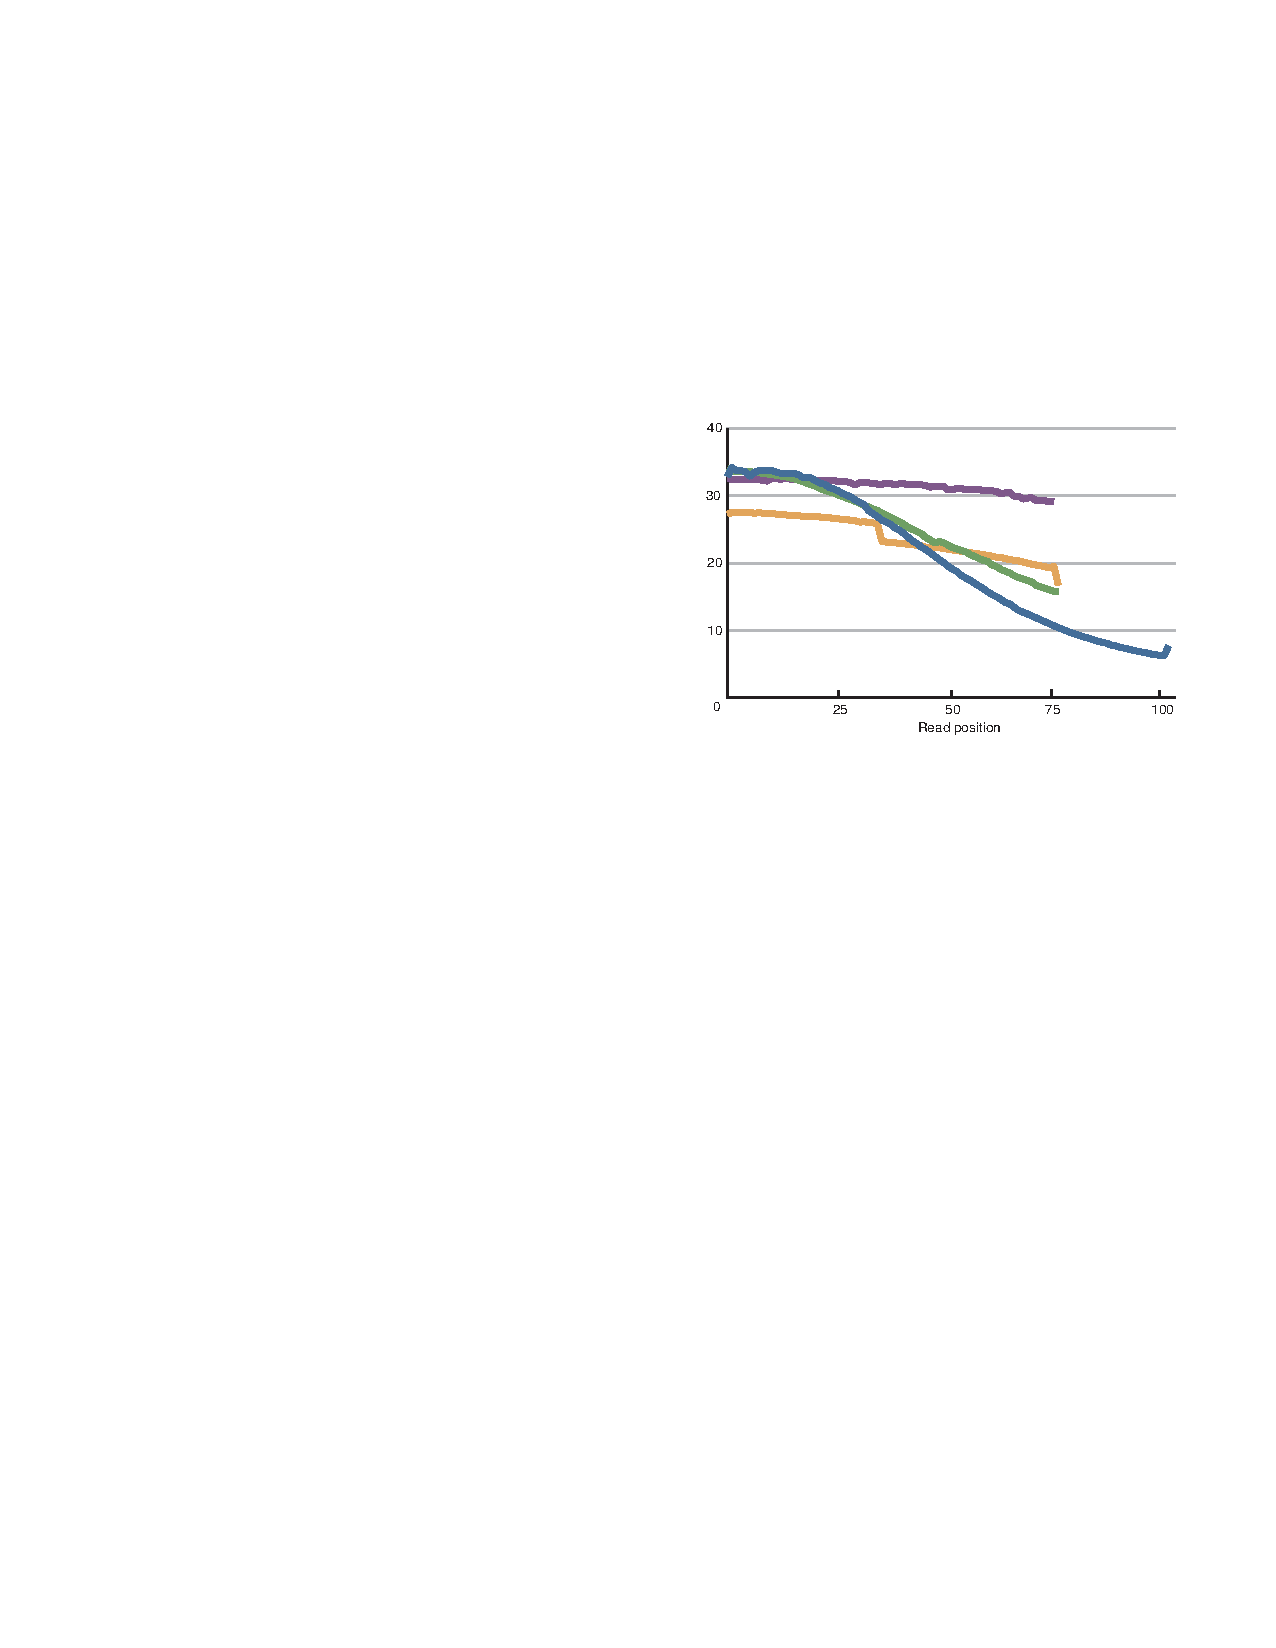
\includegraphics[width=2in]{img/illumina-error-rate-by-cycle.pdf}
\newline {\tiny [Nakamura et al.]}
\begin{itemize}
\item Short-reads ($\sim 100$ bp), paired-end
\begin{itemize}
\item Read length limited by phase coherence of amplicon colonies
\end{itemize}
\item Mate-pair libraries give potential for long-range information
\item \textbf{Very} high throughput
\end{itemize}
\end{frame}
\begin{frame}
\frametitle{Generation 2 example: Illumina}
\label{sec-2-3}

   \begin{columns}[c]
   \column{2.2in} \hspace{0.1in} 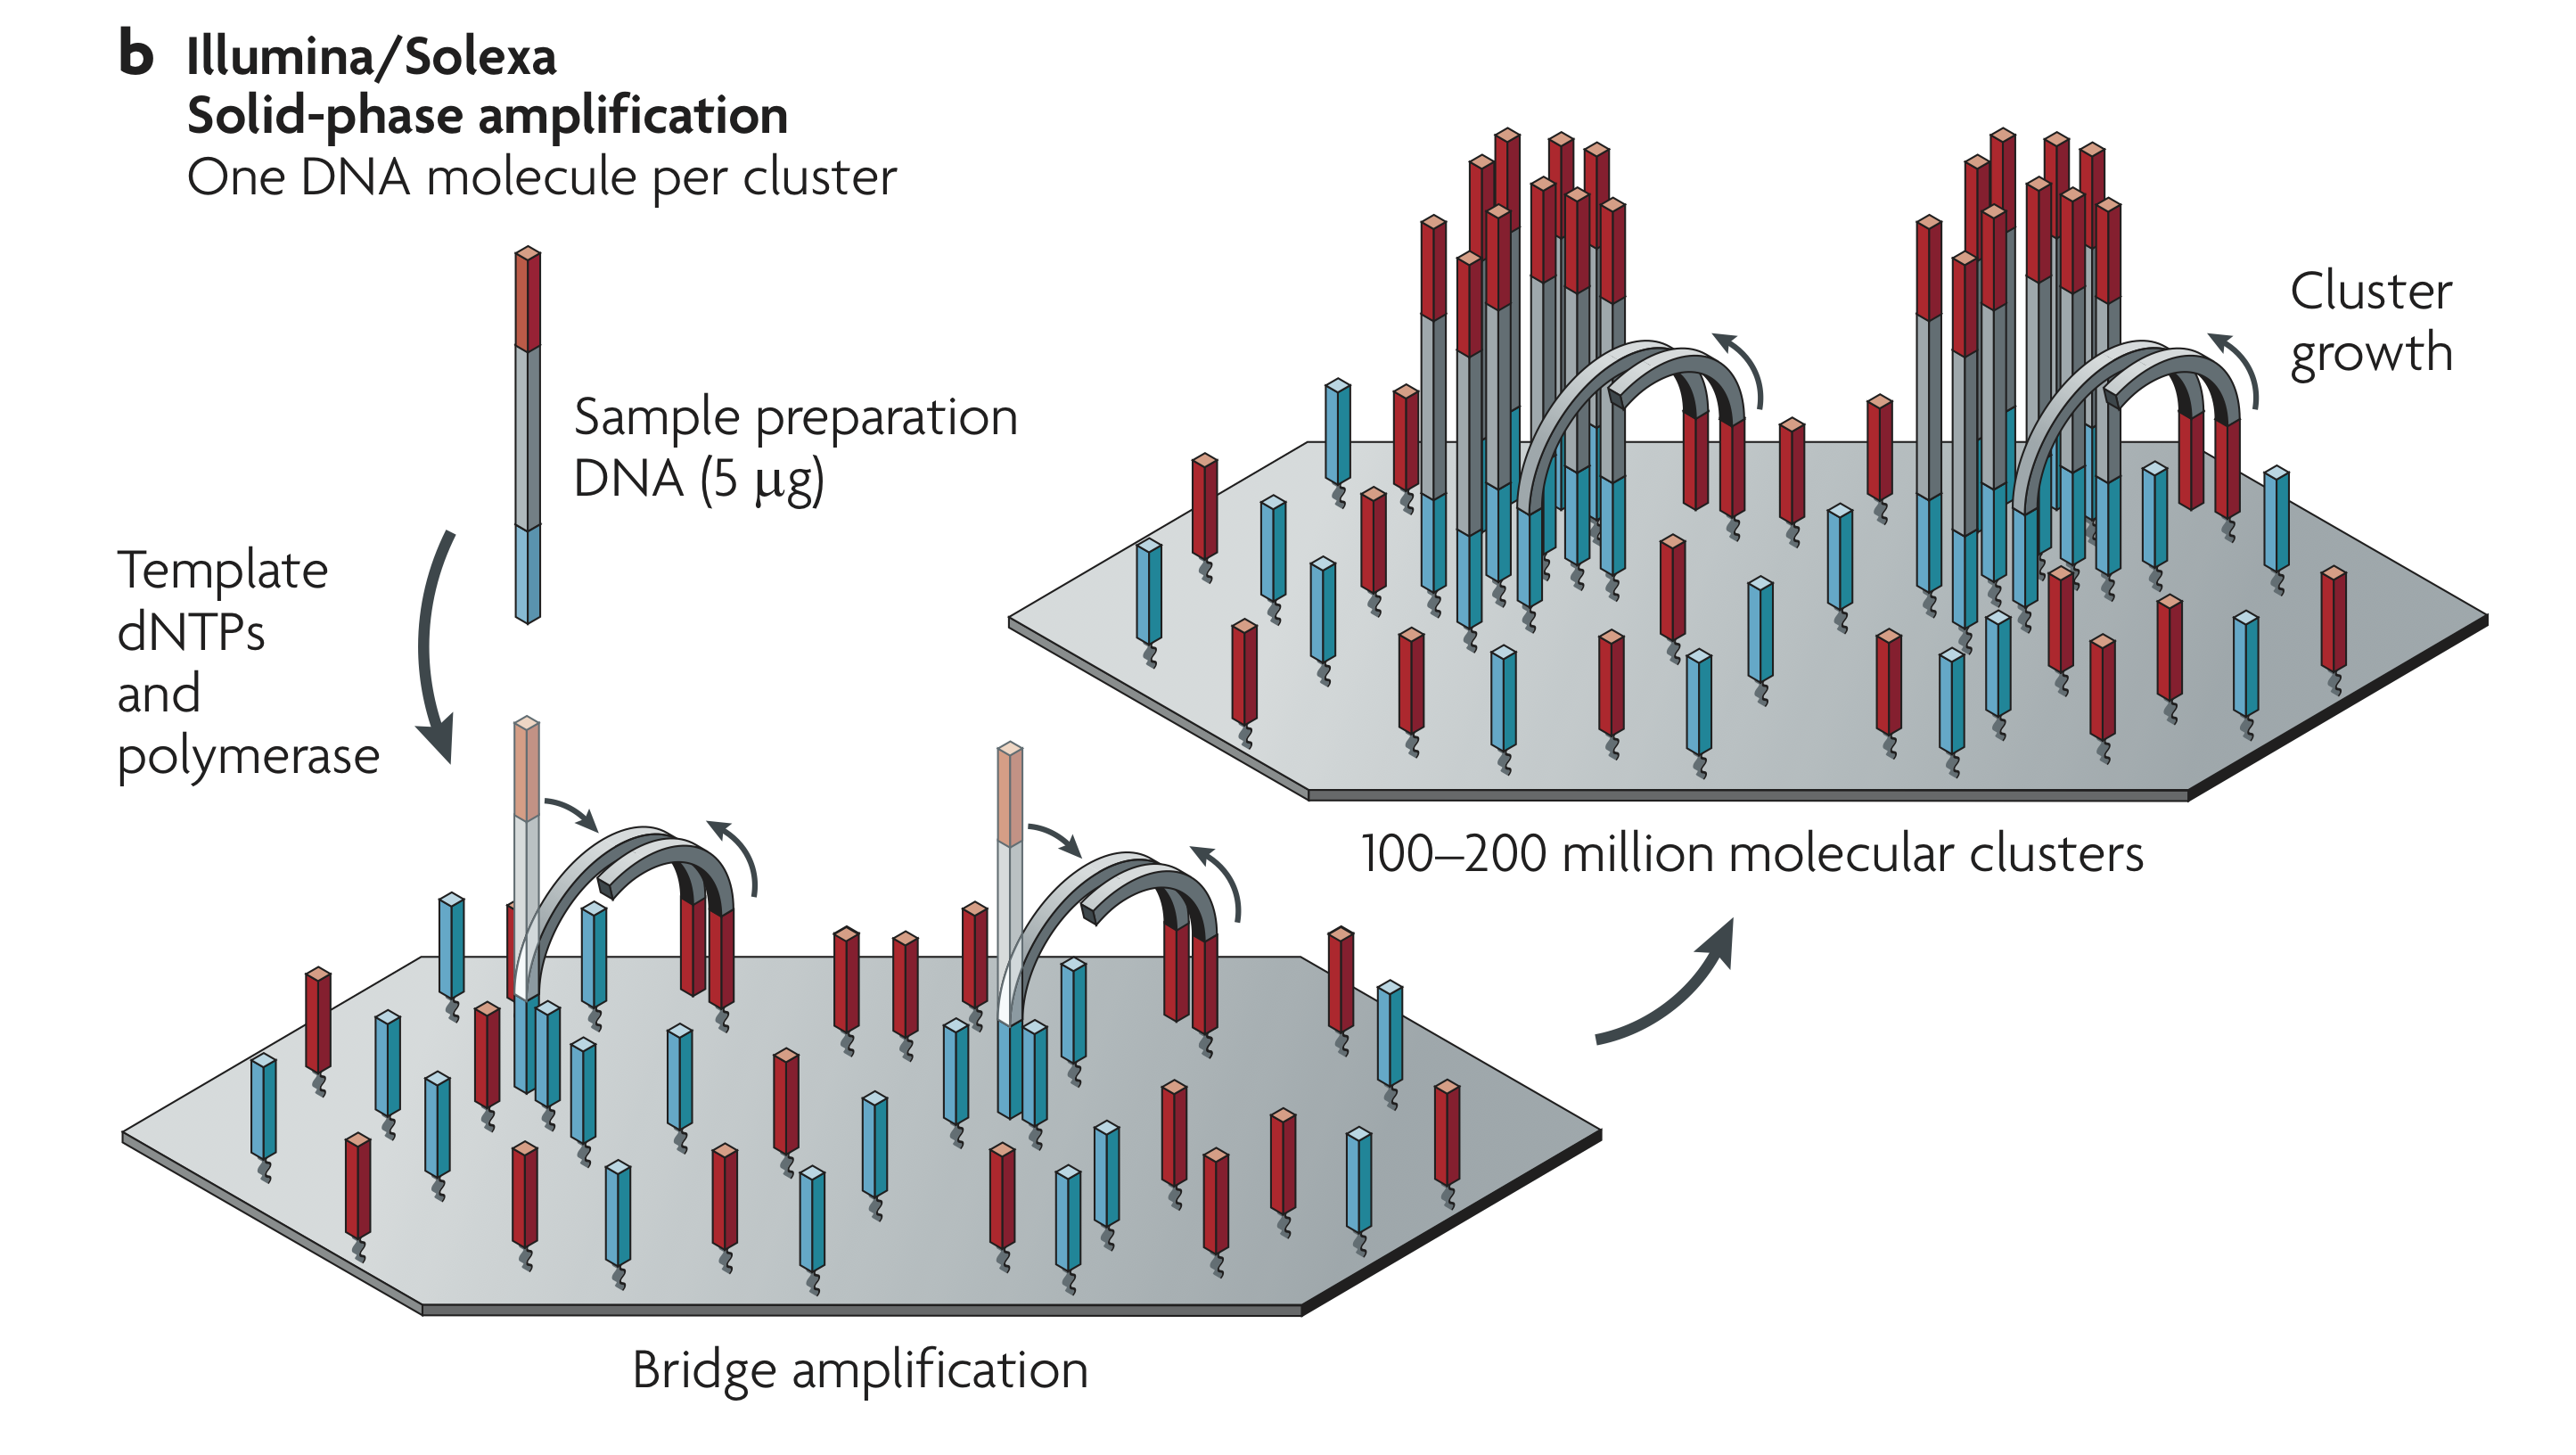
\includegraphics[width=2in]{img/illumina-amplification.png}
   \column{2.5in} 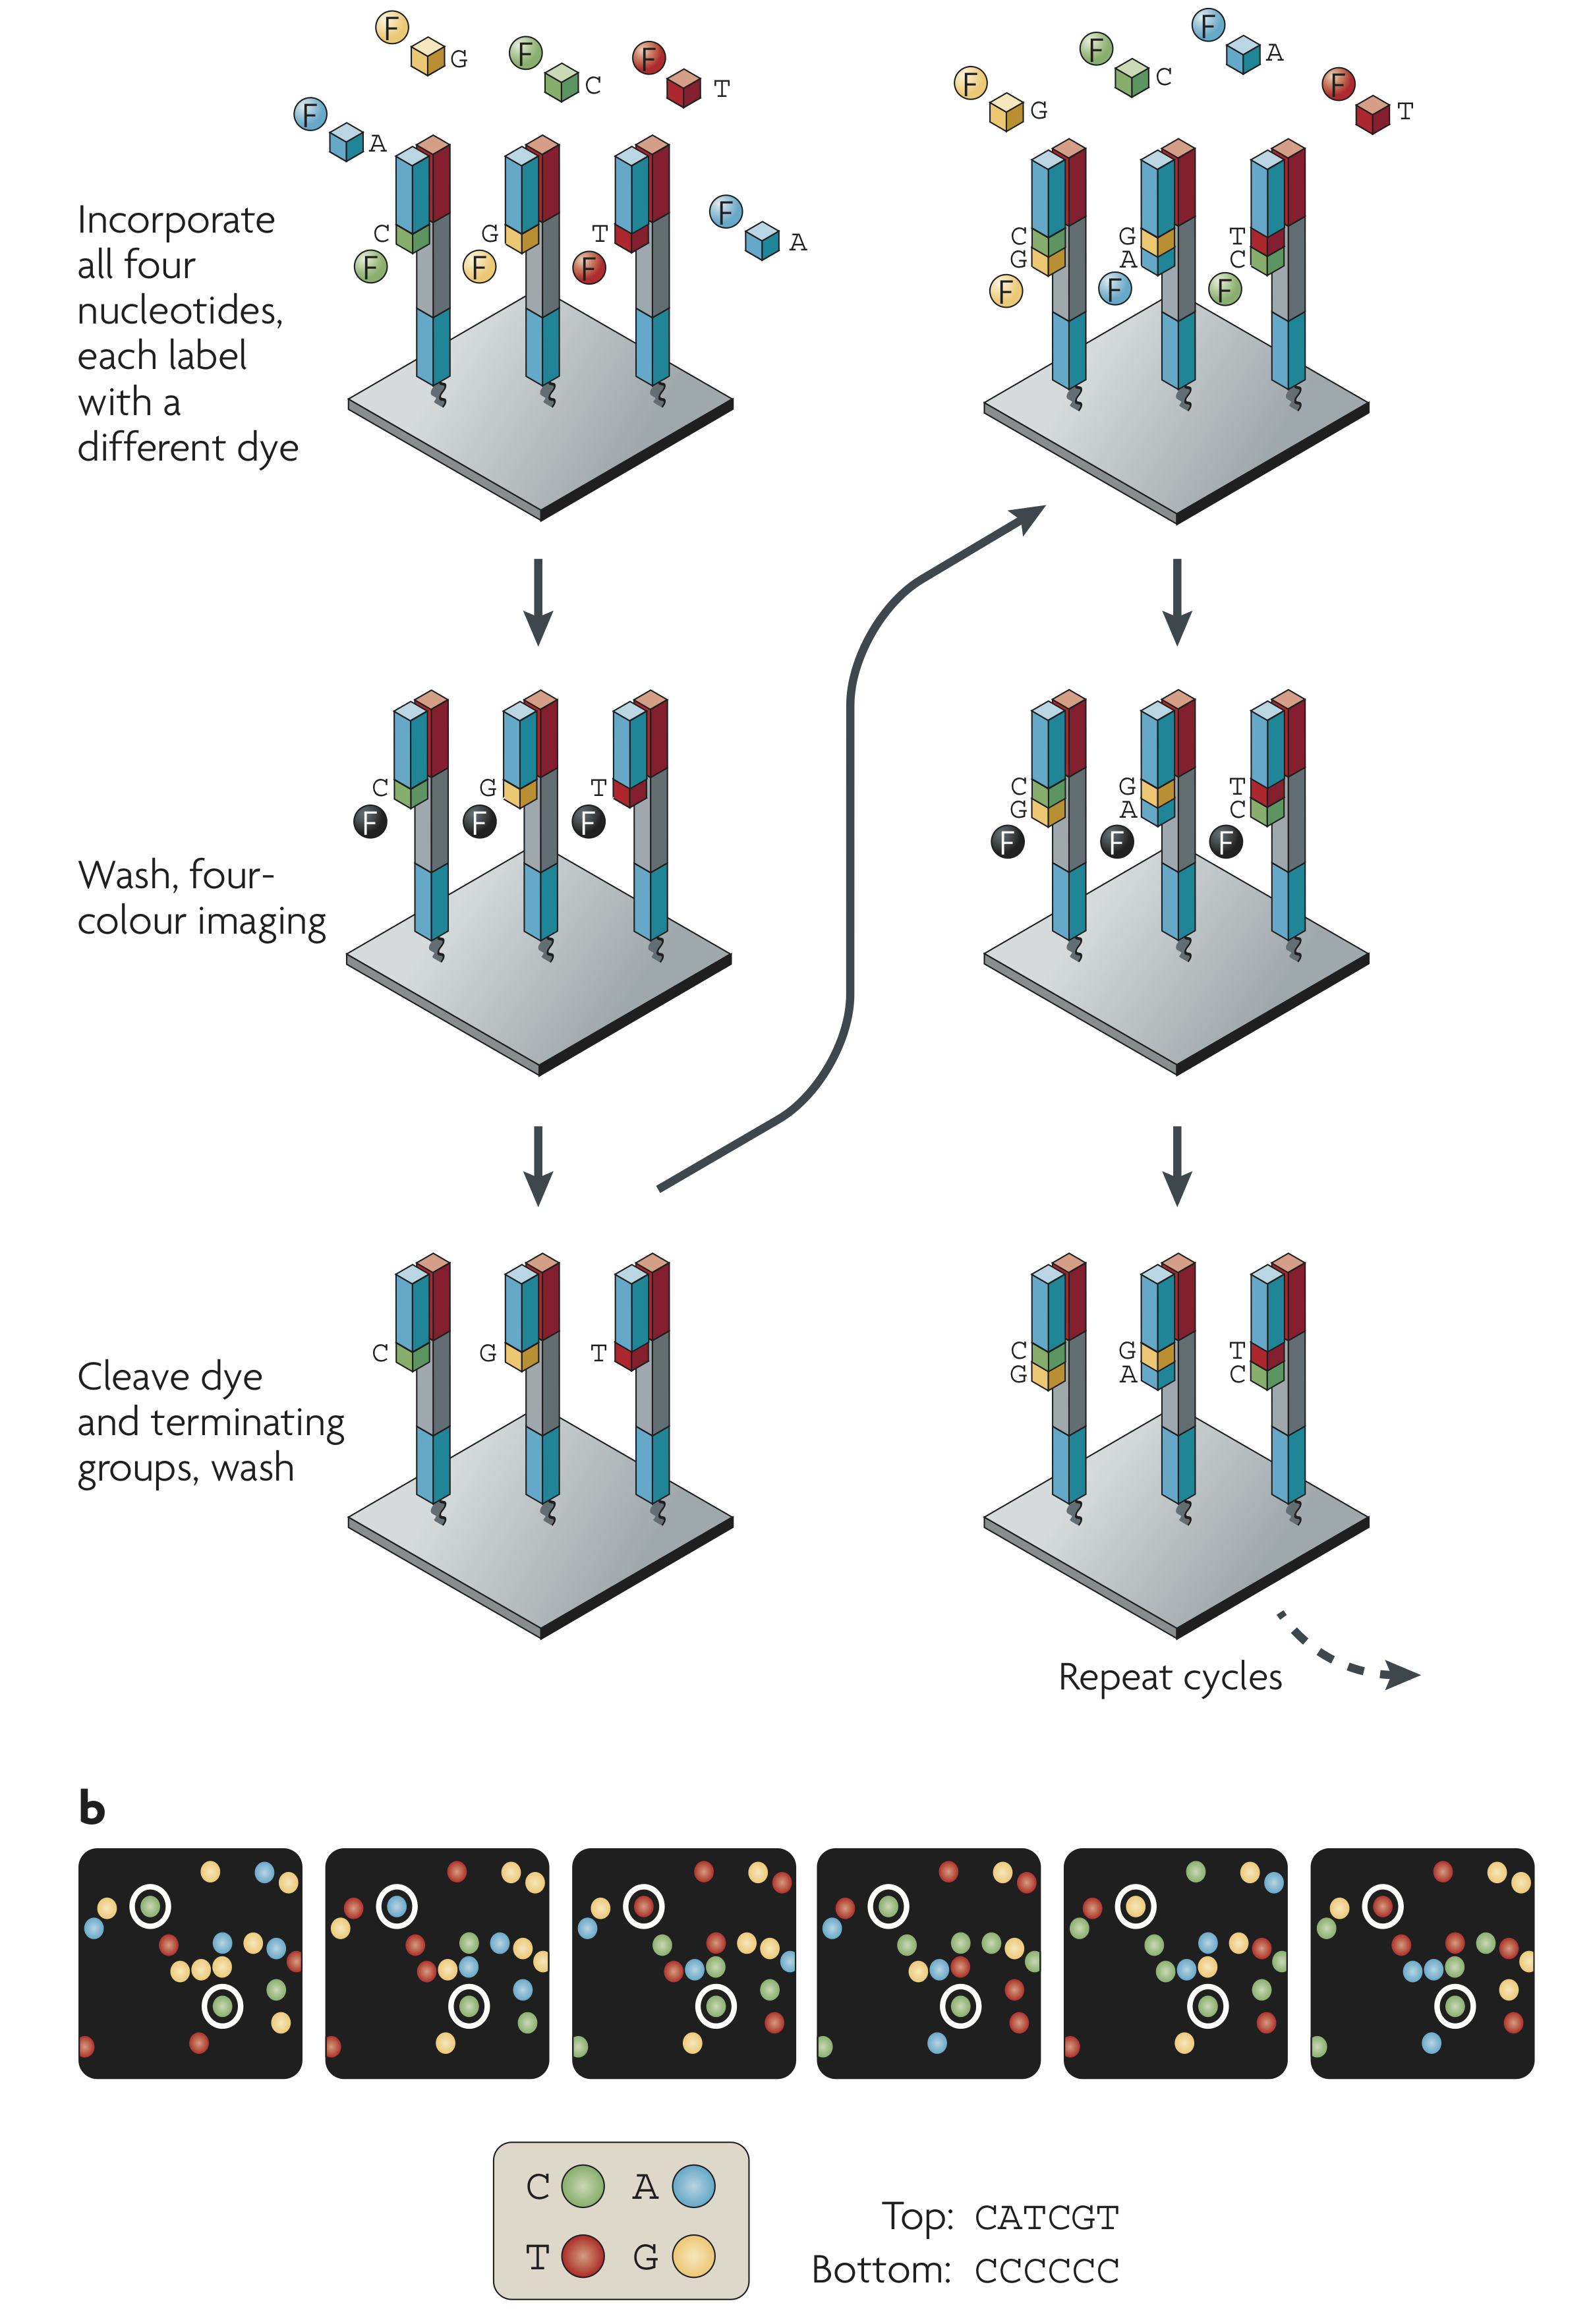
\includegraphics[width=1.8in]{img/illumina-reaction.png}
   \end{columns}

\begin{itemize}
\item Bridge PCR method for clonal amplification
\item Cyclic, reversible-terminator based chemistry
\end{itemize}
\end{frame}
\begin{frame}
\frametitle{Generation 3: High-throughput long-read technologies}
\label{sec-2-4}

   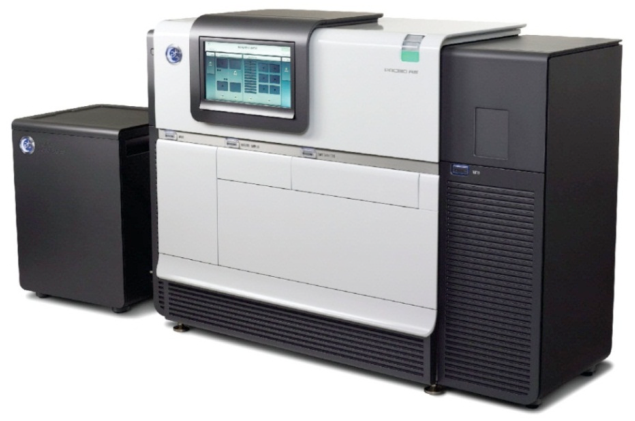
\includegraphics[width=3in]{img/RS.pdf}
   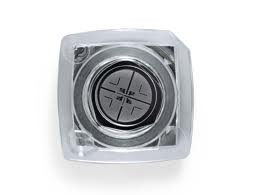
\includegraphics[width=2in]{img/smrtcell.jpeg}

   PacBio SMRT\R sequencing
\begin{itemize}
\item Very long reads (C2 chemistry mean > 3000bp; XL: > 5000bp)
\item High throughput
\end{itemize}
\end{frame}
\section{PacBio SMRT\R Sequencing}
\label{sec-3}
\begin{frame}

  \sectionpage
\end{frame}
\begin{frame}
\frametitle{SMRT\R = ``single molecule, real time''}
\label{sec-3-1}

   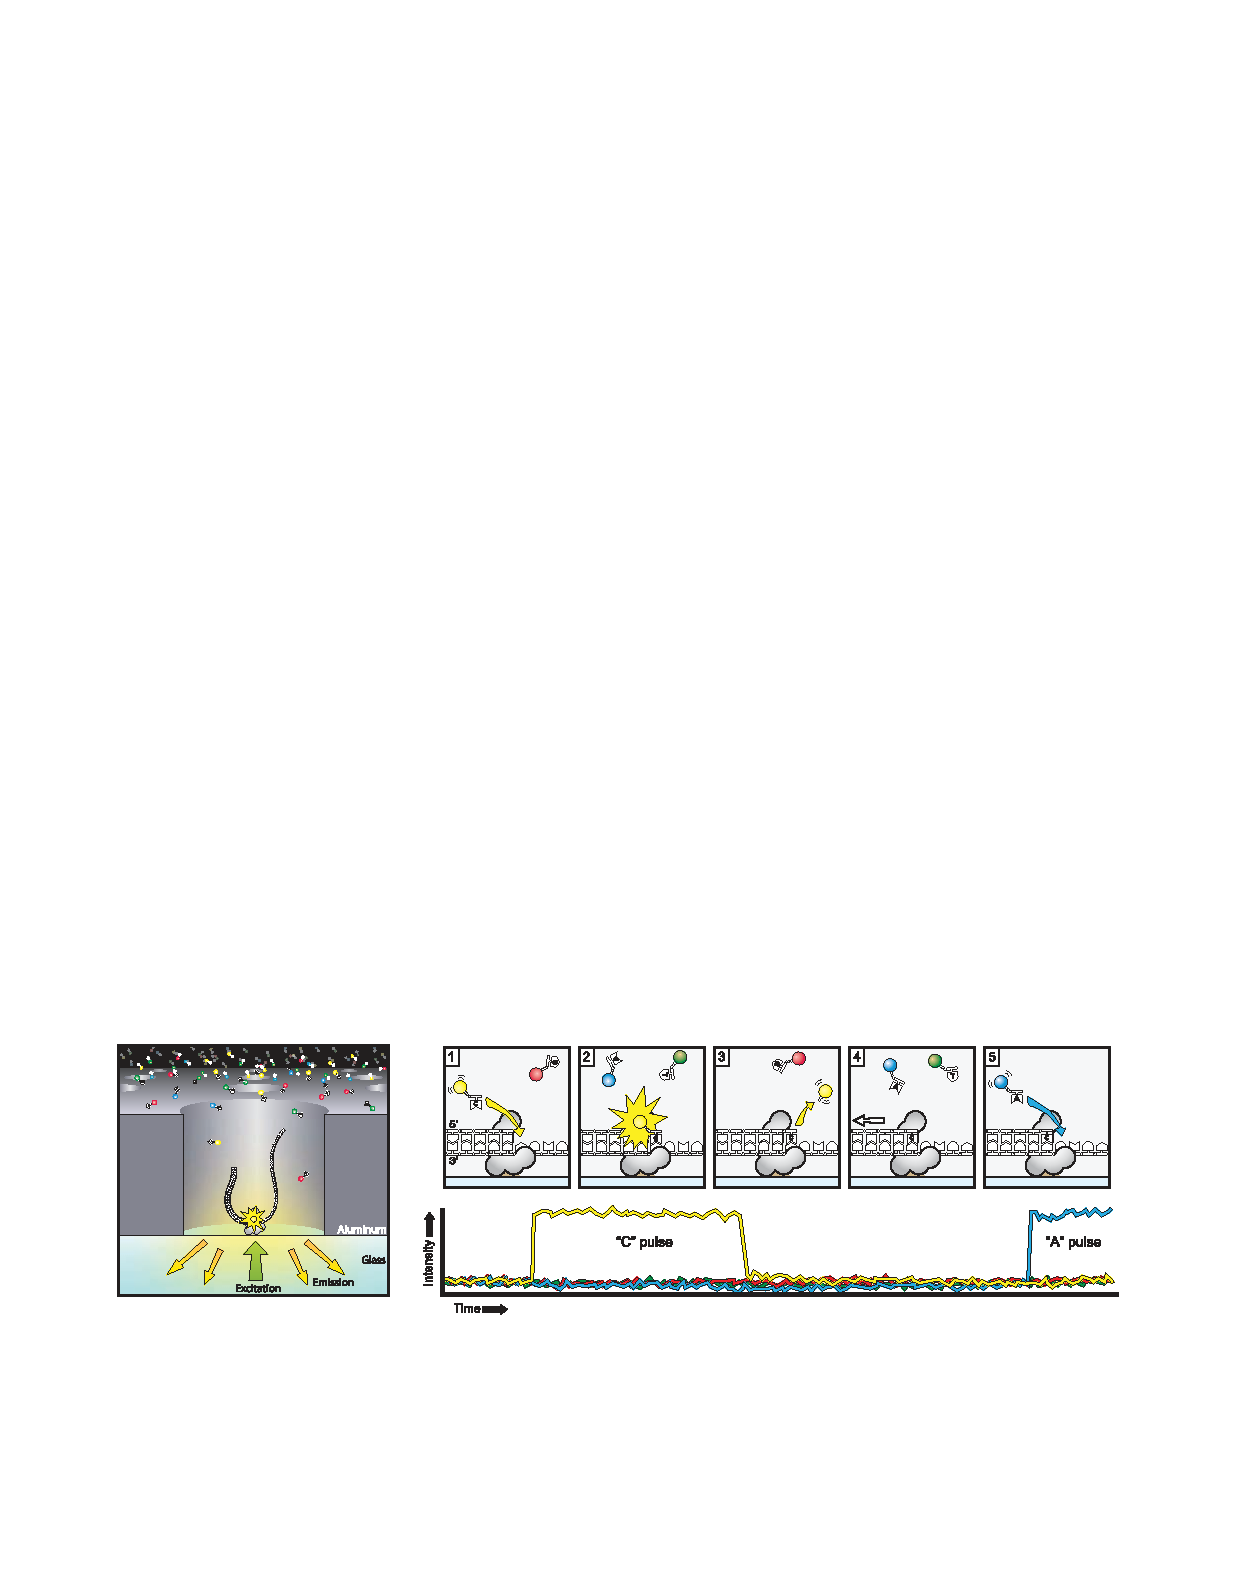
\includegraphics[width=4.5in]{img/smrt-cartoon.pdf}
   \newline {\tiny [Eid, 2009]}
\begin{itemize}
\item Polymerases immobilized in Zero-Mode Waveguides
\item DNA sequencing reaction watched in real time using
     fluorescent-labeled nucleotides
\end{itemize}
\end{frame}
\begin{frame}
\frametitle{Long, and very long, reads: history}
\label{sec-3-2}

   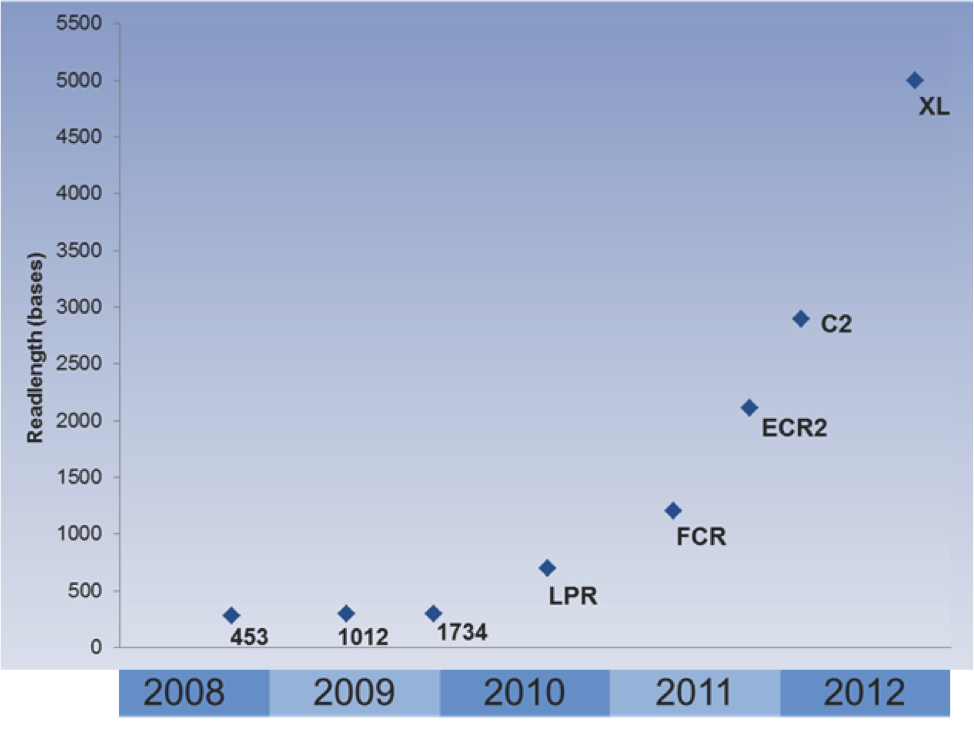
\includegraphics[width=4.2in]{img/readlength-timeline.png}
\end{frame}
\begin{frame}
\frametitle{Long, and very long, reads: C2}
\label{sec-3-3}

   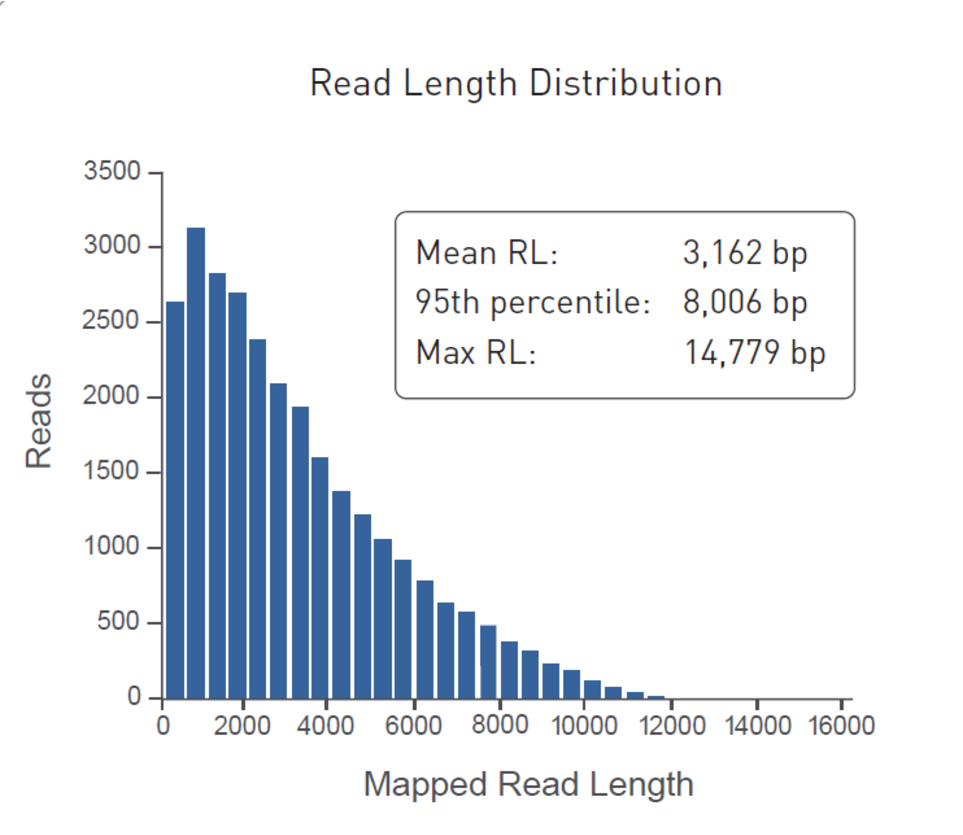
\includegraphics[width=3.8in]{img/c2-readlengths.pdf}
\end{frame}
\begin{frame}
\frametitle{From photon counts to base calls: \textbf{primary} analysis}
\label{sec-3-4}

   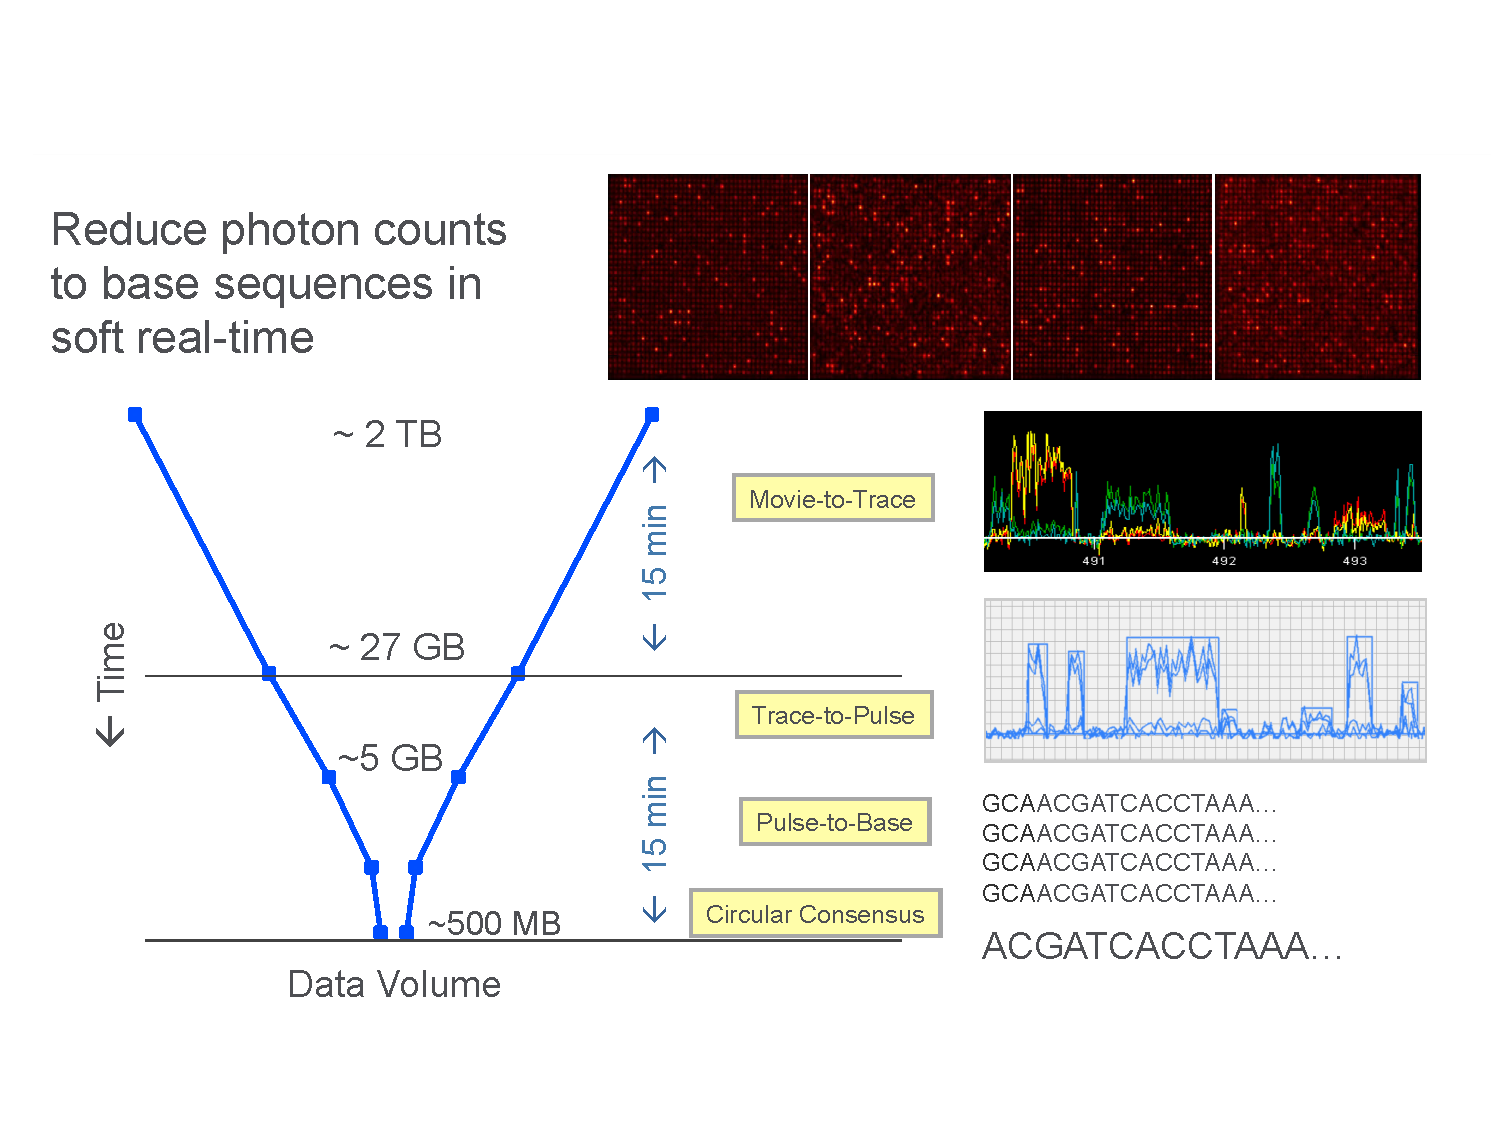
\includegraphics[width=4.5in]{img/primary-reduction.pdf}
    \newline {\tiny [Credit: Jim Labrenz]}
\end{frame}
\begin{frame}
\frametitle{From bases to actionable information: \textbf{secondary} analysis}
\label{sec-3-5}

   \vspace*{\bigskip}
   \hspace*{2em}
   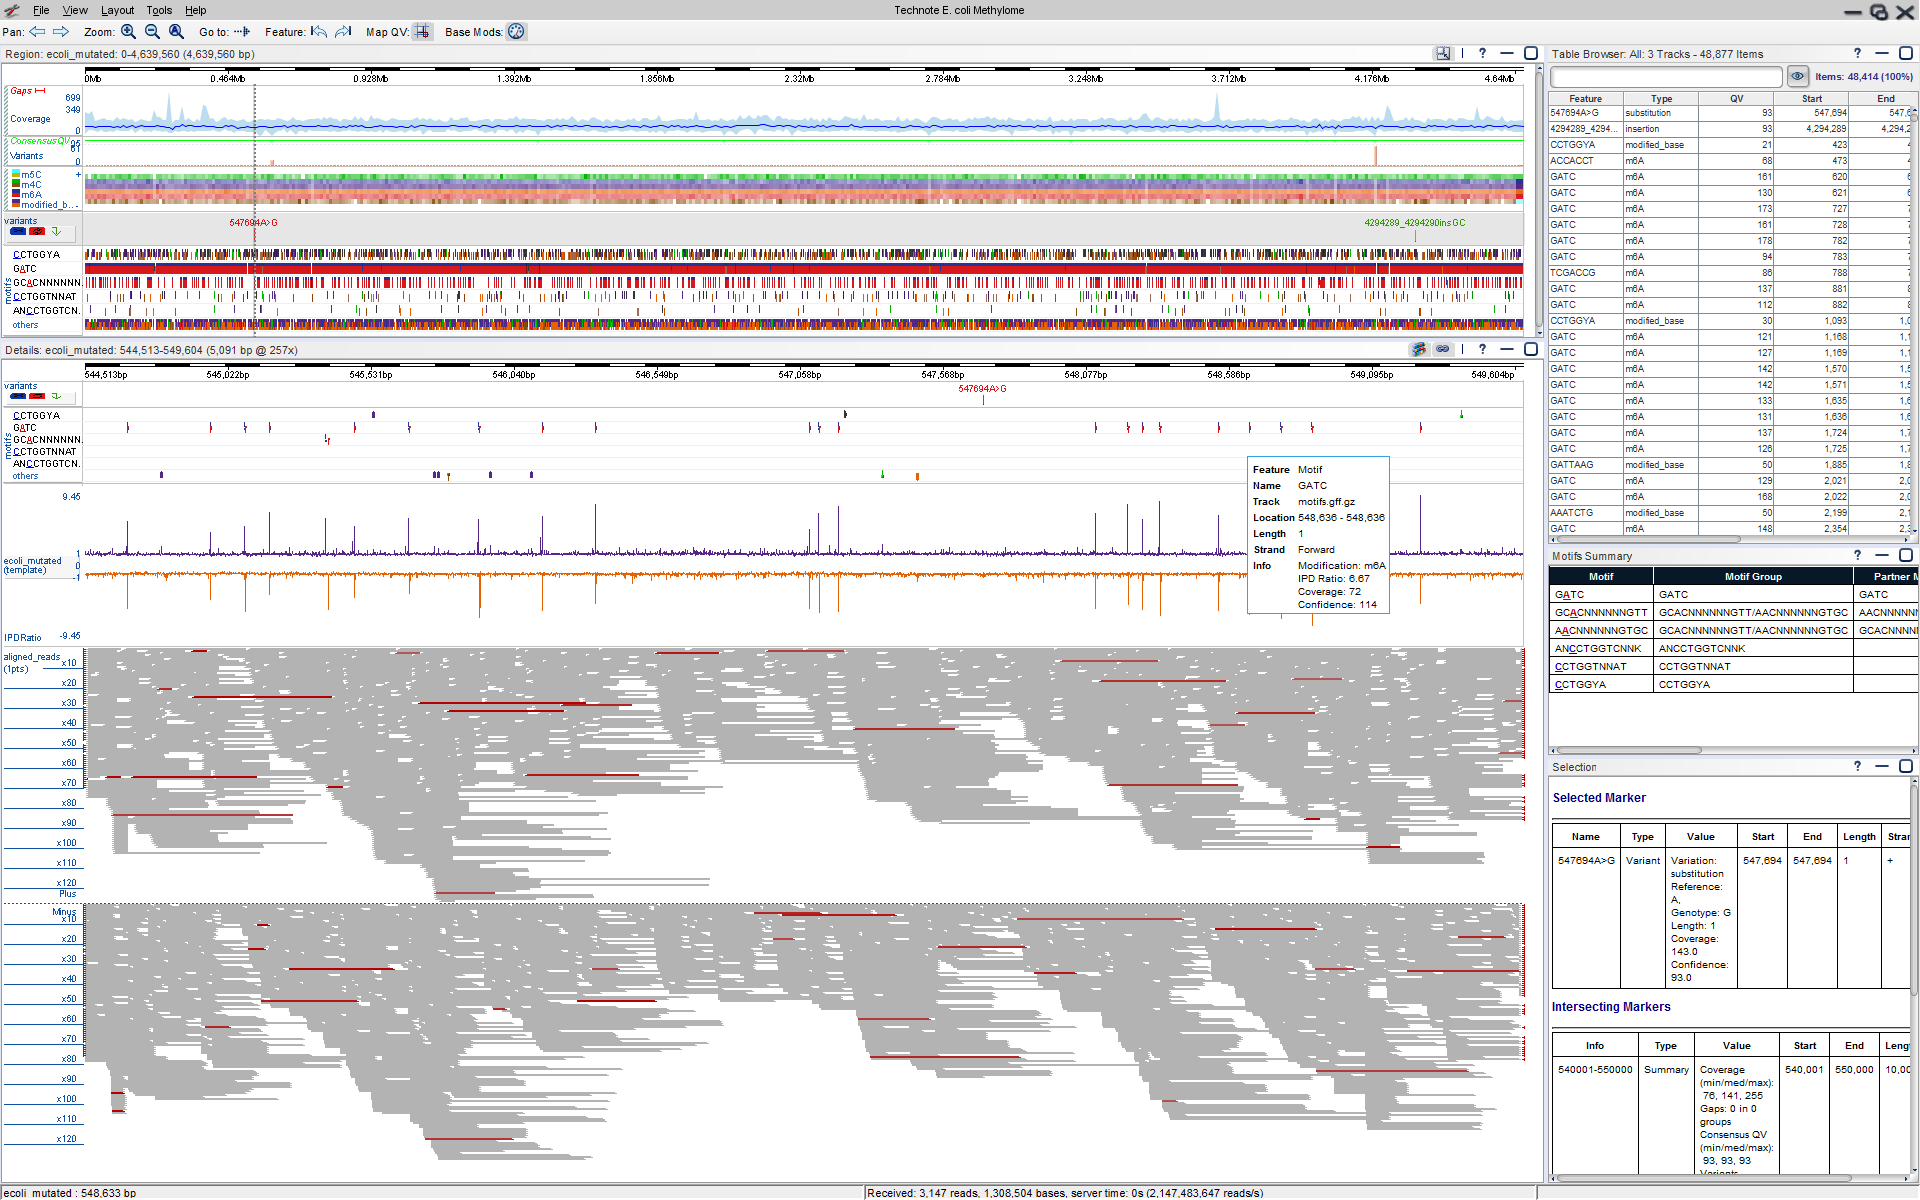
\includegraphics[width=3.6in]{img/smrtview.png}
\begin{columns} % cols
\label{sec-3-5-1}
\begin{column}{0.5\textwidth}
%% left
\label{sec-3-5-1-1}

\begin{itemize}
\item Variant calling
\item Phasing
\item \emph{De novo} genome assembly
\end{itemize}
\end{column}
\begin{column}{0.5\textwidth}
%% right
\label{sec-3-5-1-2}

\begin{itemize}
\item Methylation / base modification detection
\item Transcript analysis
\end{itemize}
\end{column}
\end{columns}
\end{frame}
\begin{frame}
\frametitle{PacBio data: error model}
\label{sec-3-6}

   \begin{figure}
   \centering
     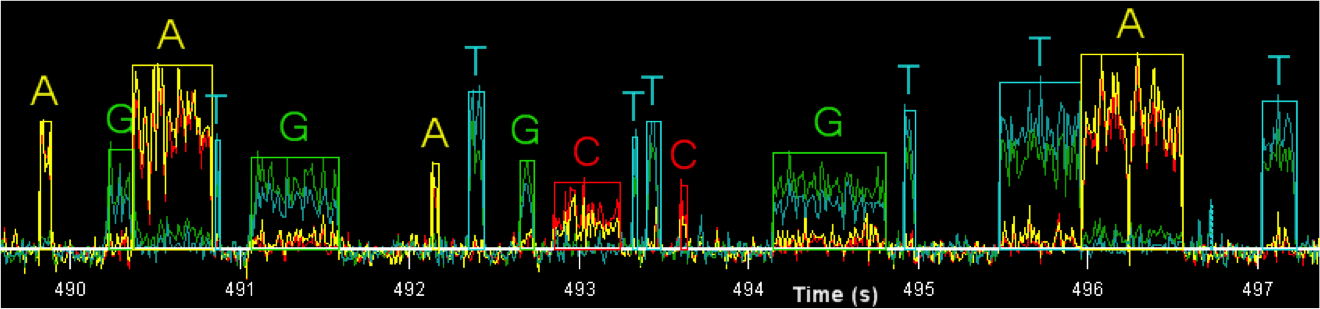
\includegraphics[width=4.5in]{img/trace.png}
   \end{figure}

\begin{itemize}
\item Errors dominated by indels
\begin{itemize}
\item Cognate extras (homopolymer expansion)
\item Noncognate extras
\item Dark pulses
\item Pulse merging (homopolymer contraction)
\end{itemize}
\item \emph{Essentially no substitutions}
\end{itemize}
\end{frame}
\begin{frame}[fragile]
\frametitle{PacBio data: data format}
\label{sec-3-7}

   \verb~bas.h5~ file contains a lot more than just basecalls.  Basecaller
   provides metrics indicating areas of uncertainty.  ``Breadcrumbs''


\begin{center}
\begin{tabular}{lrrrlr}
 Base  &  Insertion  &  Substitution  &  Deletion  &  Deletion  &  Merge  \\
       &         QV  &            QV  &        QV  &  Tag       &     QV  \\
\hline
 A     &          8  &            12  &        16  &  N         &     14  \\
 T     &          2  &            12  &         5  &  T         &    100  \\
 T     &         11  &            30  &         4  &  G         &     25  \\
 G     &         12  &            30  &        11  &  A         &     11  \\
 G     &          3  &            30  &        16  &  N         &     27  \\
 C     &          6  &            30  &        16  &  N         &     19  \\
 C     &          3  &            19  &         3  &  C         &     21  \\
 G     &          2  &            21  &         4  &  G         &     22  \\
\end{tabular}
\end{center}



   $$QV = -10 \log_{10} p_{error}$$
\end{frame}
\section{A genome assembly primer}
\label{sec-4}
\begin{frame}

   \sectionpage
\end{frame}
\begin{frame}
\frametitle{Shotgun sequencing and assembly}
\label{sec-4-1}

   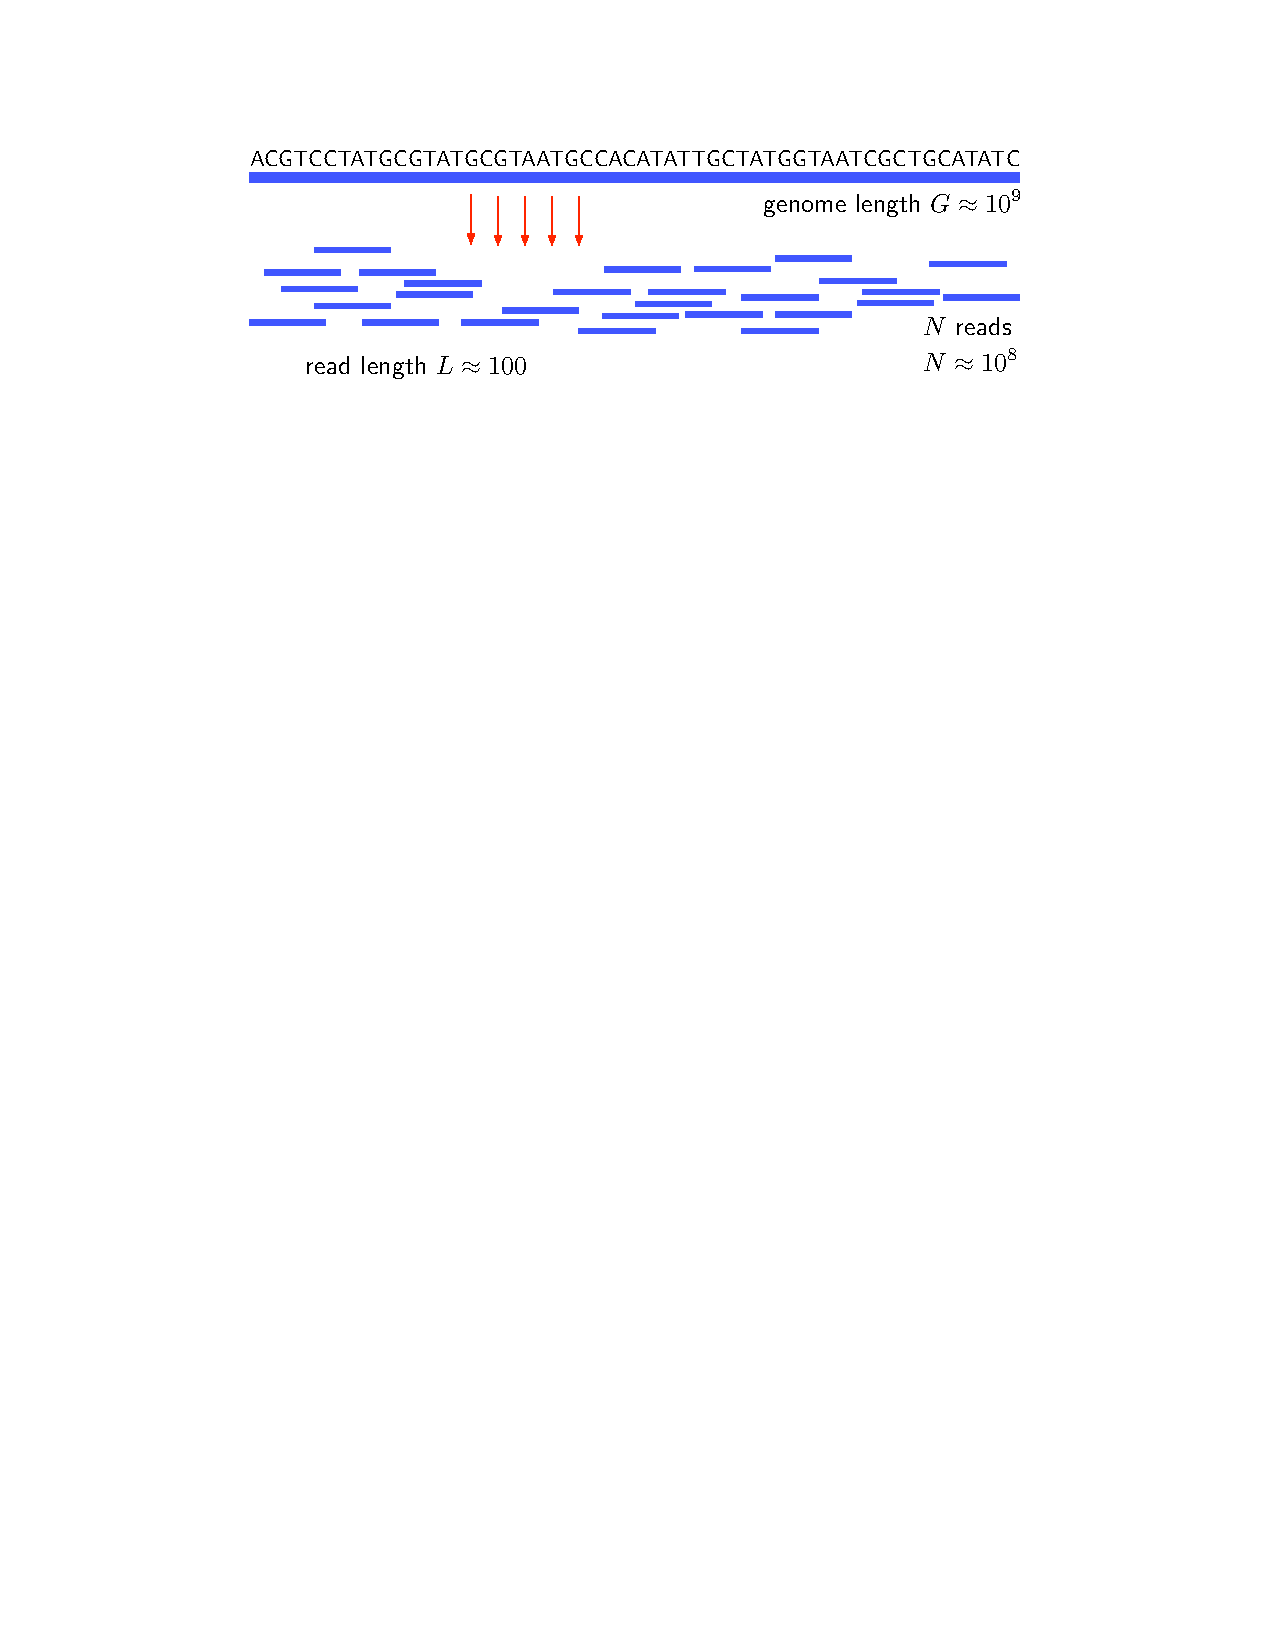
\includegraphics[width=4.5in]{img/shotgun.pdf}
\newline \tiny [Credit: David Tse]
\end{frame}
\begin{frame}
\frametitle{Shotgun sequencing and assembly}
\label{sec-4-2}

   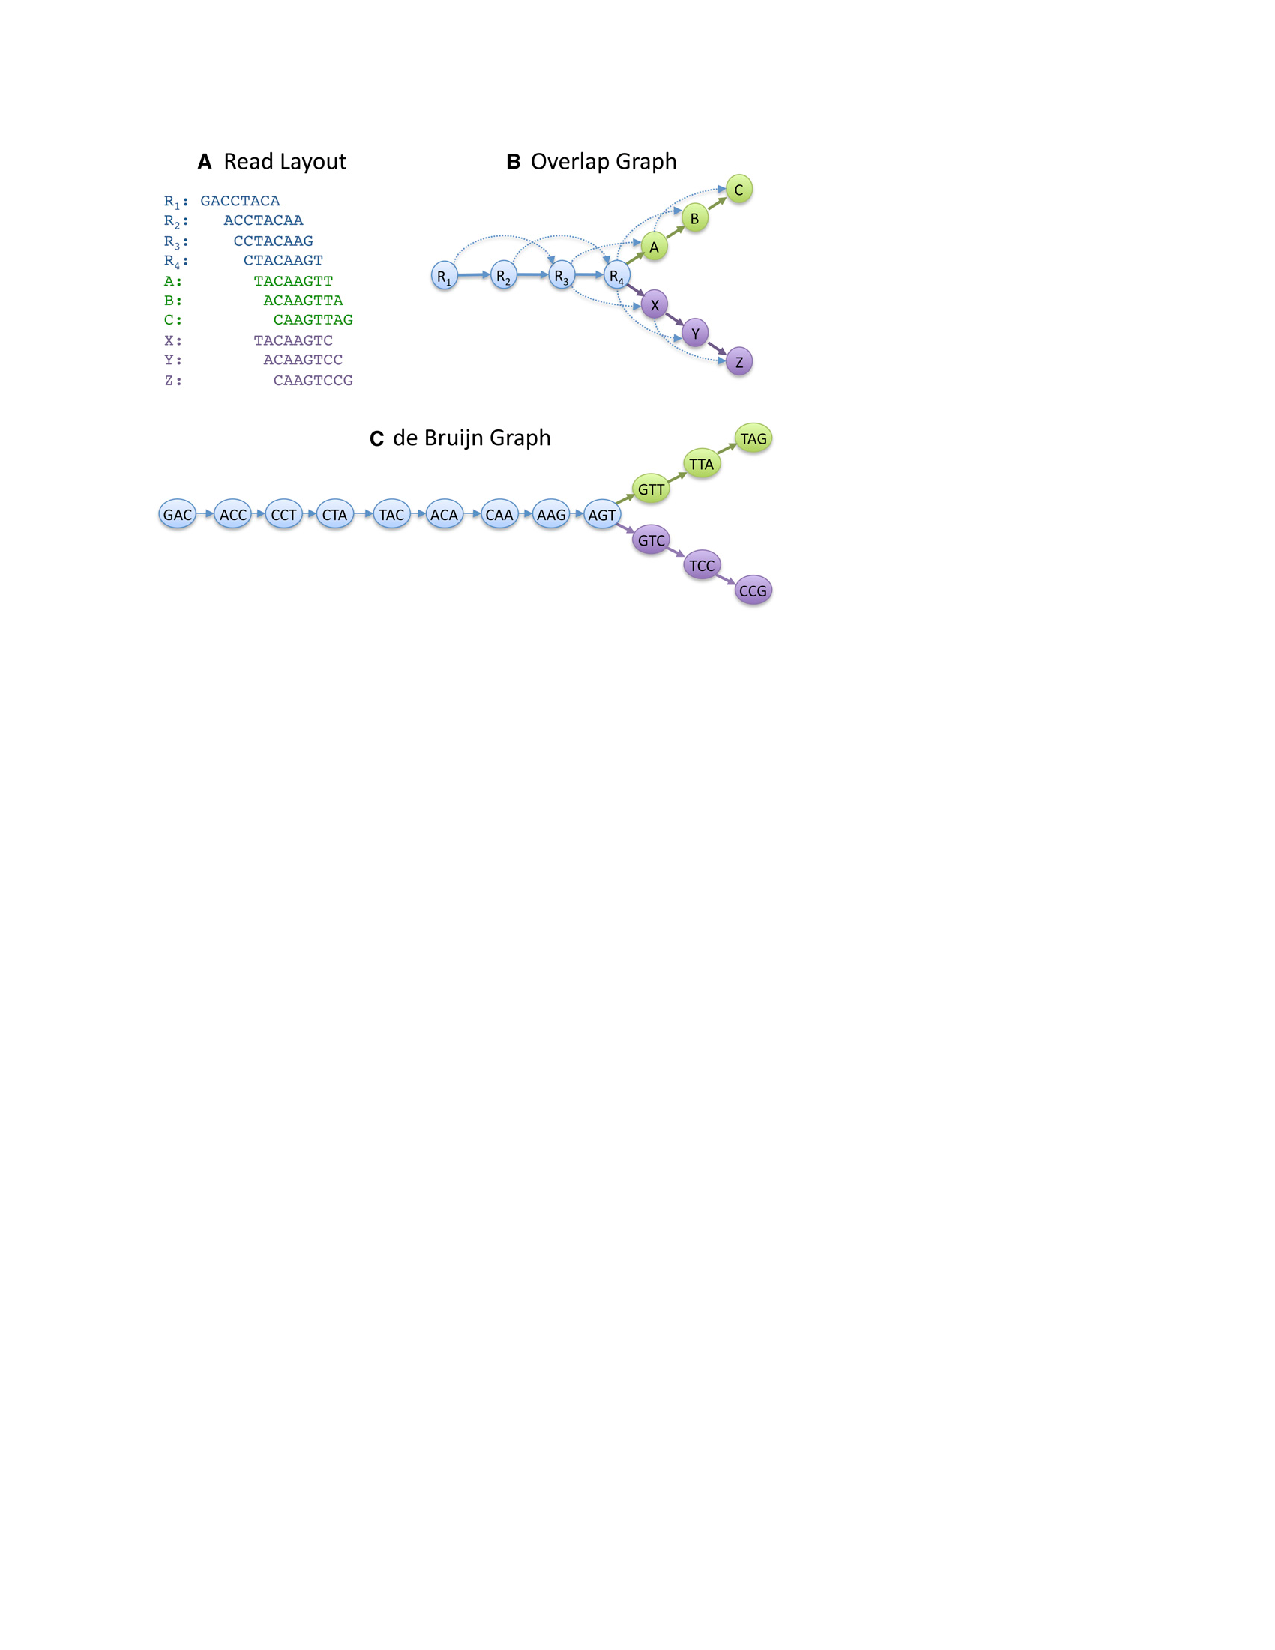
\includegraphics[width=4in]{img/overlap-graphs.pdf}
\newline \tiny [Credit: Mike Schatz]
\end{frame}
\begin{frame}
\frametitle{Lander-Waterman model (1988)}
\label{sec-4-3}

   Idealization of genome assembly.  Letting $L$ denote readlength,
   $G$ genome size, and $C$ coverage, main results:
\begin{block}{Expected number of contigs (ideal)}
\label{sec-4-3-1}

    $$\mathrm{E}[\mathrm{NumContigs}]  = L^{-1}GC e^{-C}$$
\end{block}
\begin{block}{Expected contig length (ideal)}
\label{sec-4-3-2}

    $$\mathrm{E}[\mathrm{ContigLength}] = LC^{-1}(e^{C} - 1)$$

    Predicts that long reads are better, but sufficient short read
    coverage would be just as good.  \textbf{However\ldots{}}
\end{block}
\end{frame}
\begin{frame}
\frametitle{Long repeats are everywhere}
\label{sec-4-4}
\begin{columns} % FOO
\label{sec-4-4-1}
\begin{column}{0.5\textwidth}
\begin{block}{Human mobile elements}
\label{sec-4-4-1-1}

    \vspace{0.2in}
    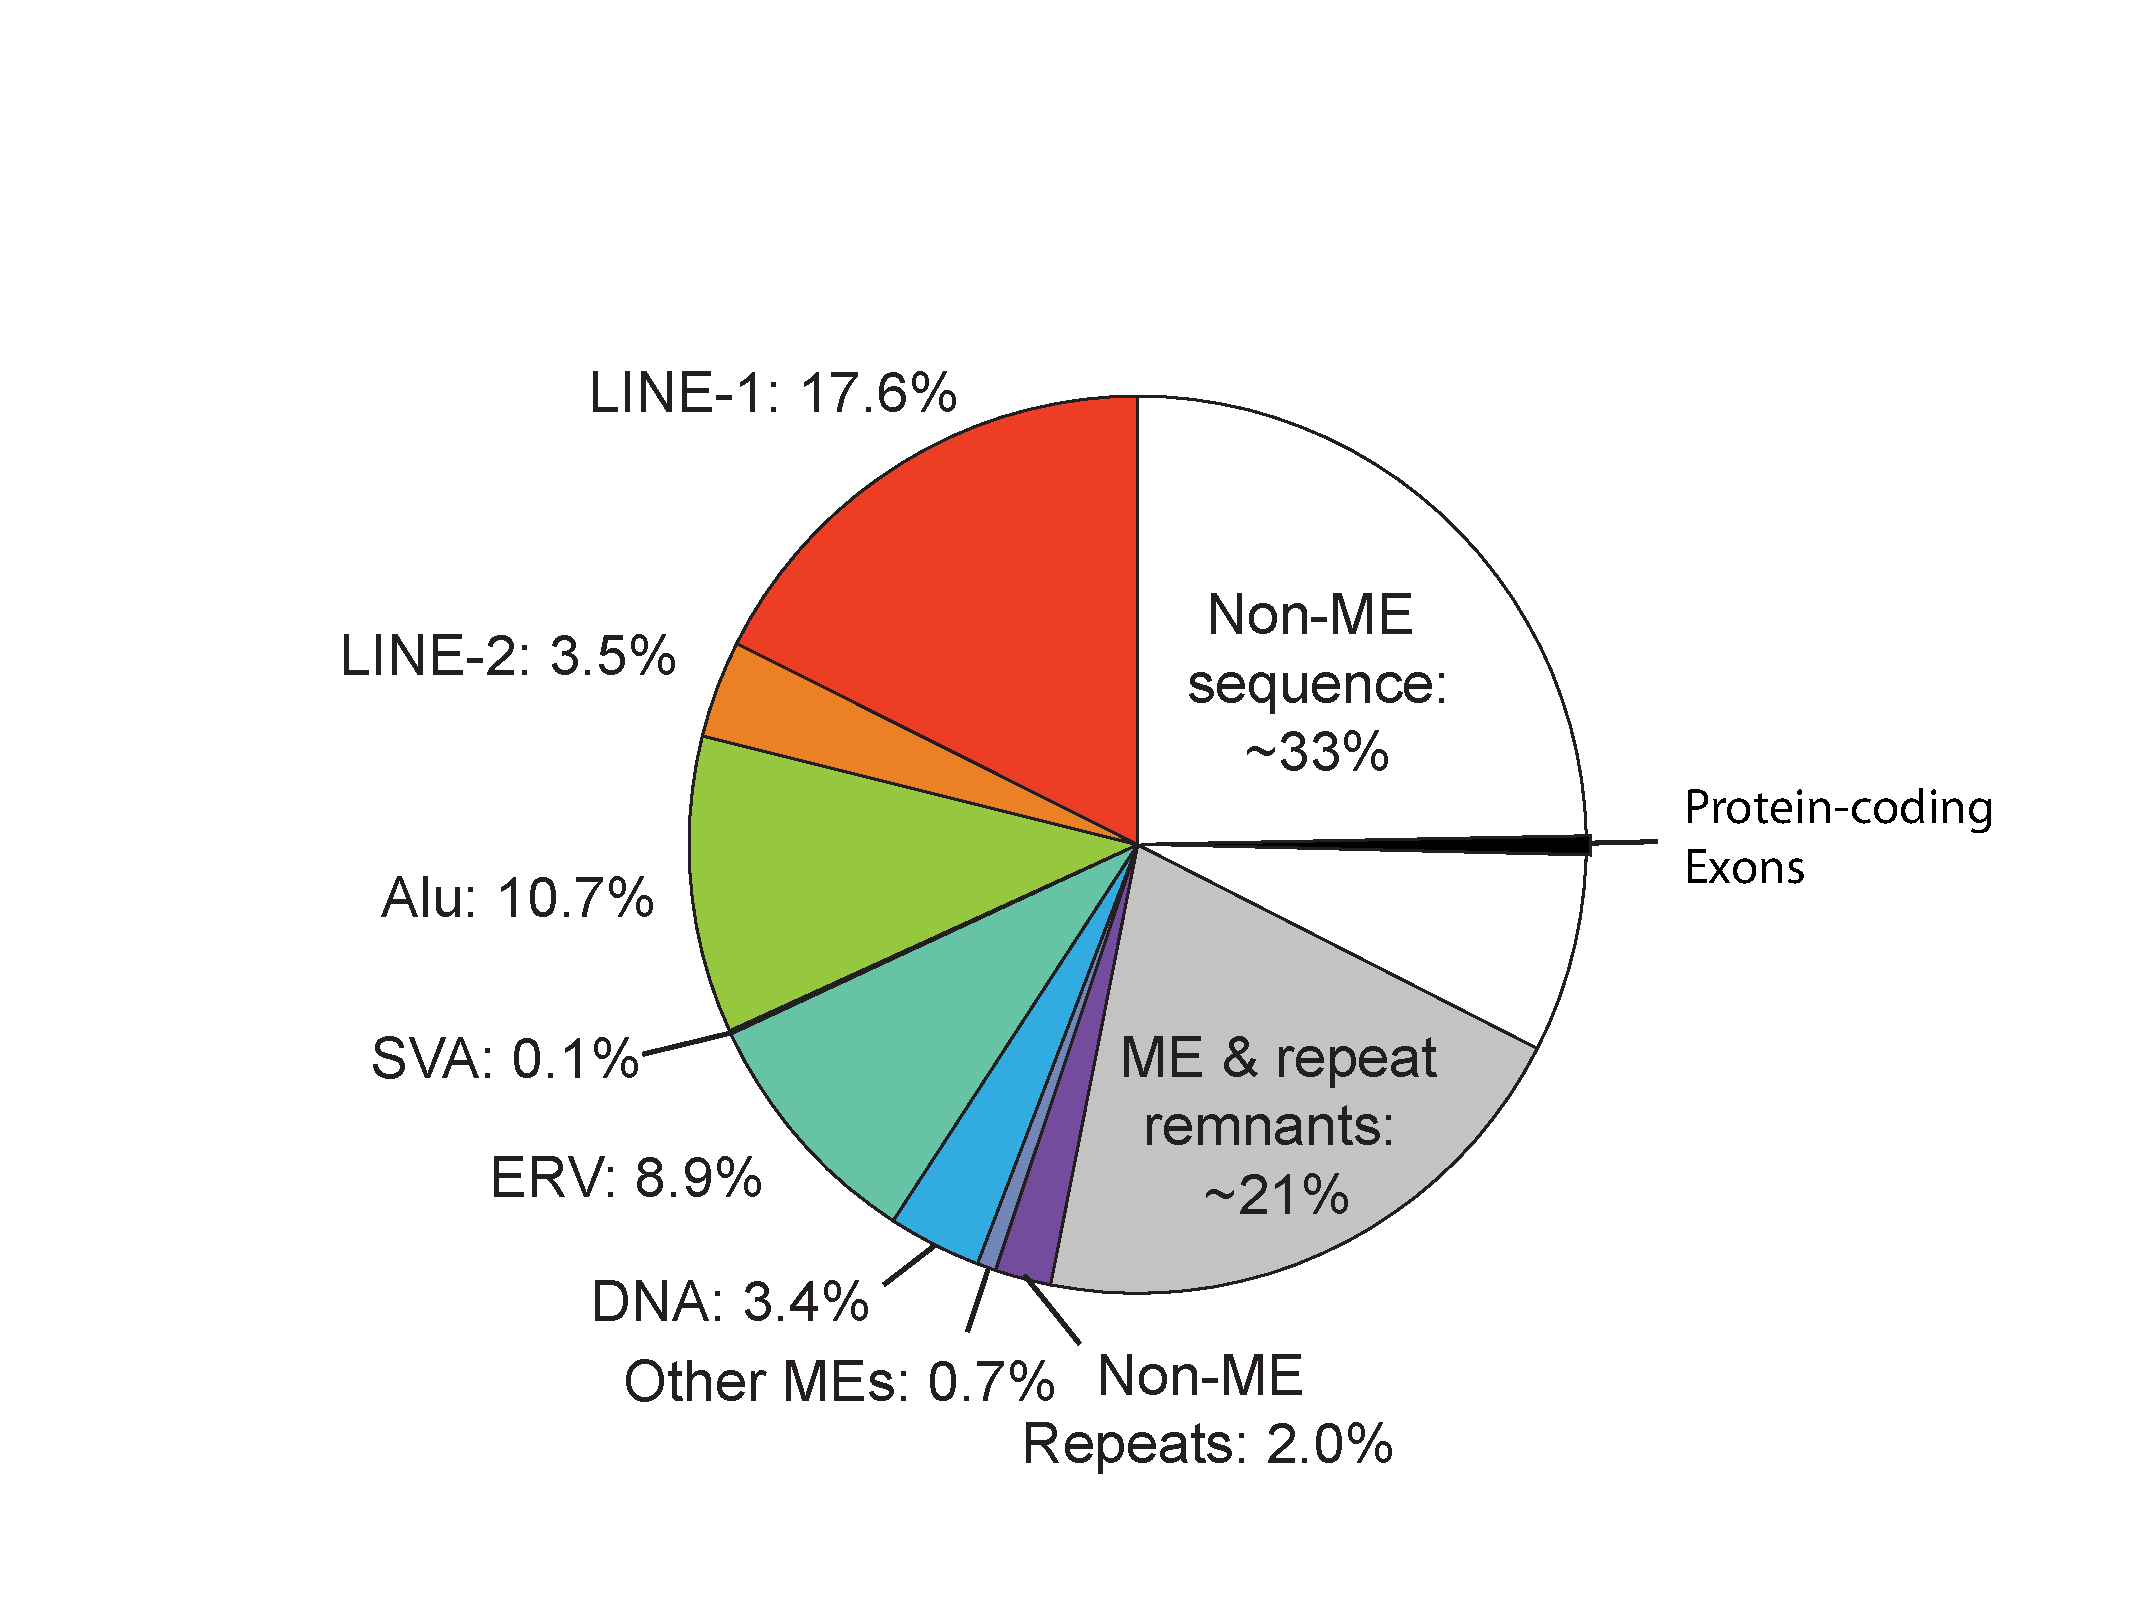
\includegraphics[width=2.3in]{img/witherspoon-mobile-elements.pdf}
    \newline
    \tiny [Credit: David Witherspoon]
\end{block}
\end{column}
\begin{column}{0.5\textwidth}
\begin{block}{\emph{E Coli} long repeats}
\label{sec-4-4-1-2}

     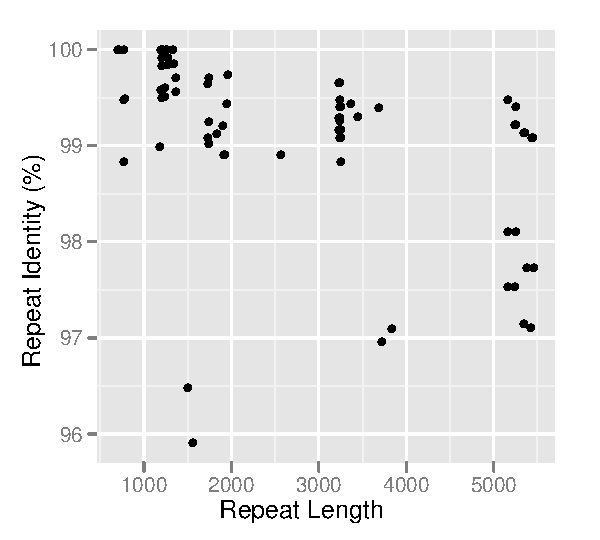
\includegraphics[width=2in]{img/ecoli-repeats.pdf}
\end{block}
\end{column}
\end{columns}
%% text (ignored)
\label{sec-4-4-2}

    Long repeats stymie short read assembly:
\begin{itemize}
\item False edges introduced into overlap graph
\item \emph{Misassembly}
\item Workarounds---mate-pair, clone libraries---require more laborious sample prep
\end{itemize}
\end{frame}
\section{HGAP assembly procedure}
\label{sec-5}
\begin{frame}

   \sectionpage
\end{frame}
\begin{frame}
\frametitle{Hierarchical genome assembly procedure (HGAP)}
\label{sec-5-1}

   \hspace*{-0.2in}
   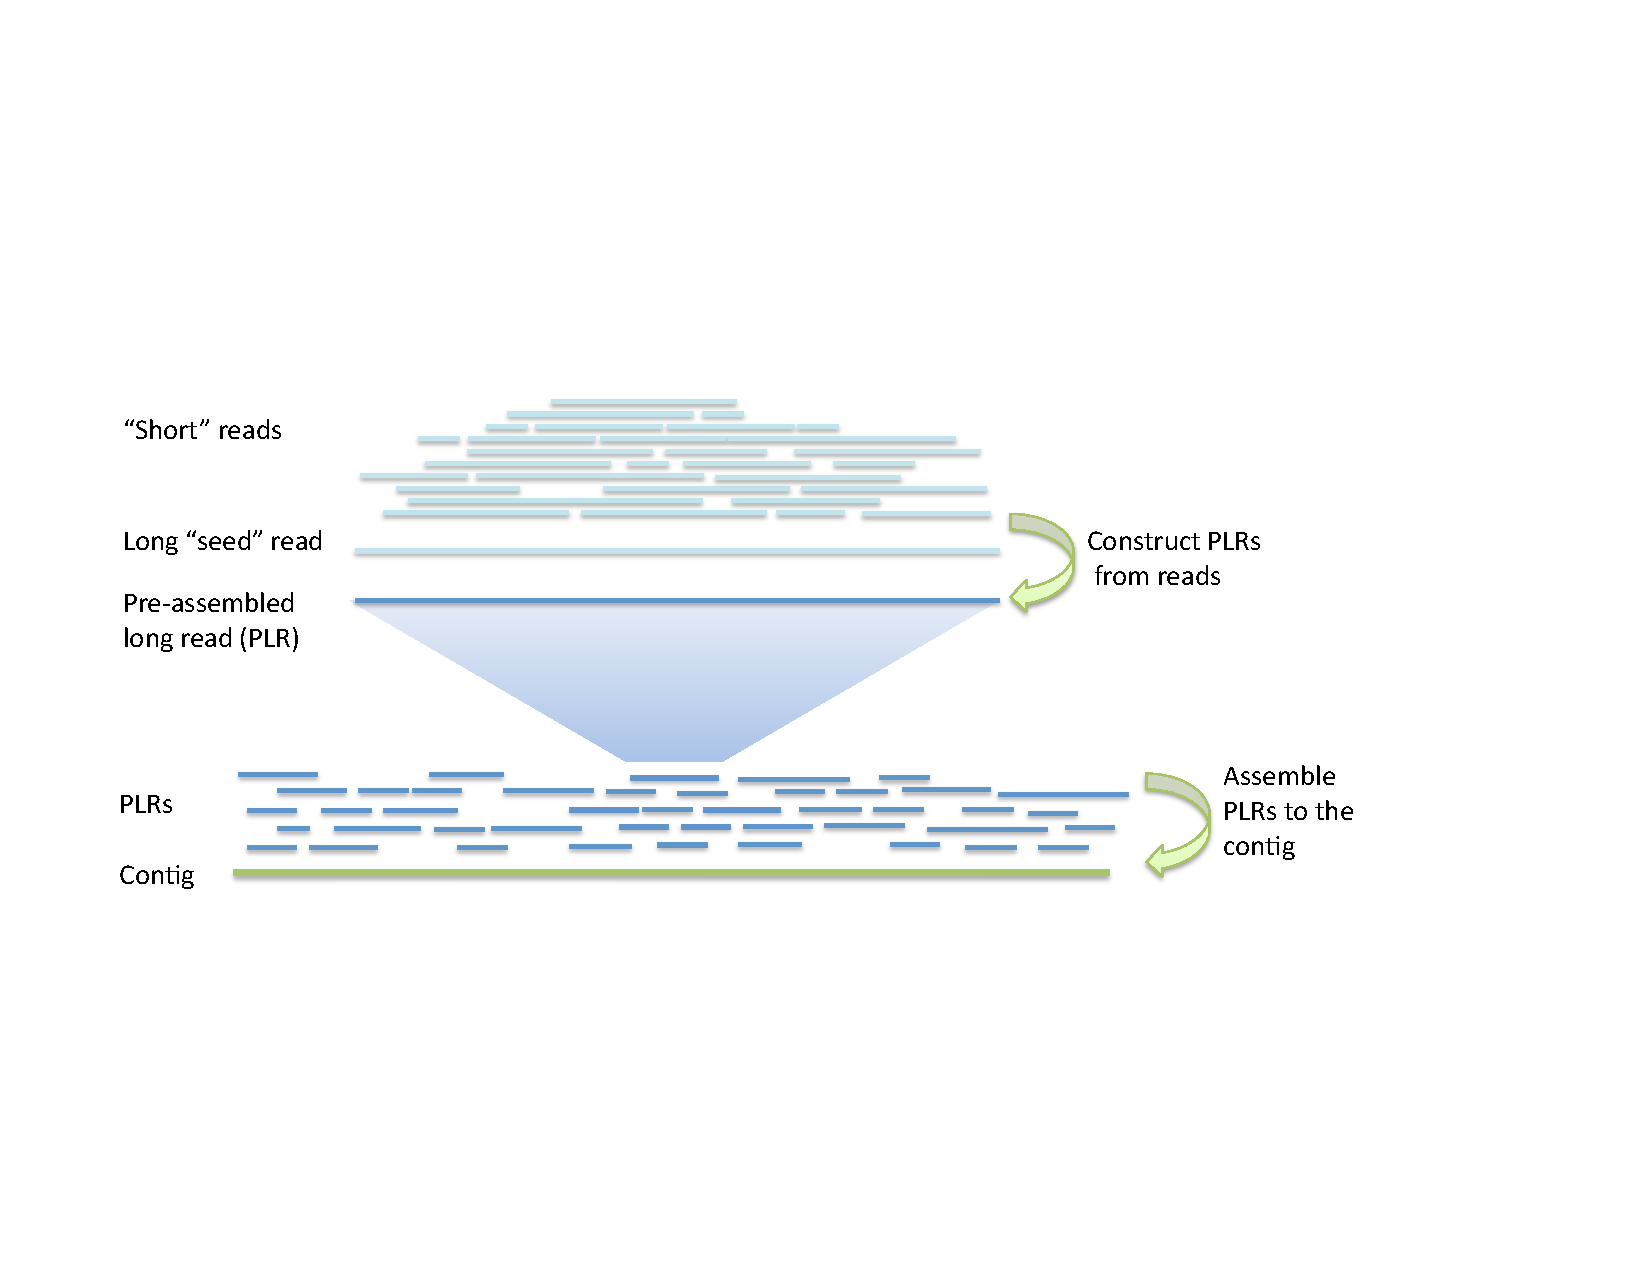
\includegraphics[width=4.75in]{img/hgap.pdf}
   \hspace*{0.4in}
\newline \tiny [Credit: Jason Chin]\hspace*{\fill}
\end{frame}
\begin{frame}
\frametitle{HGAP application: \emph{Meiothermus ruber} (JGI/DOE)}
\label{sec-5-2}

   \hspace*{-0.2in}
   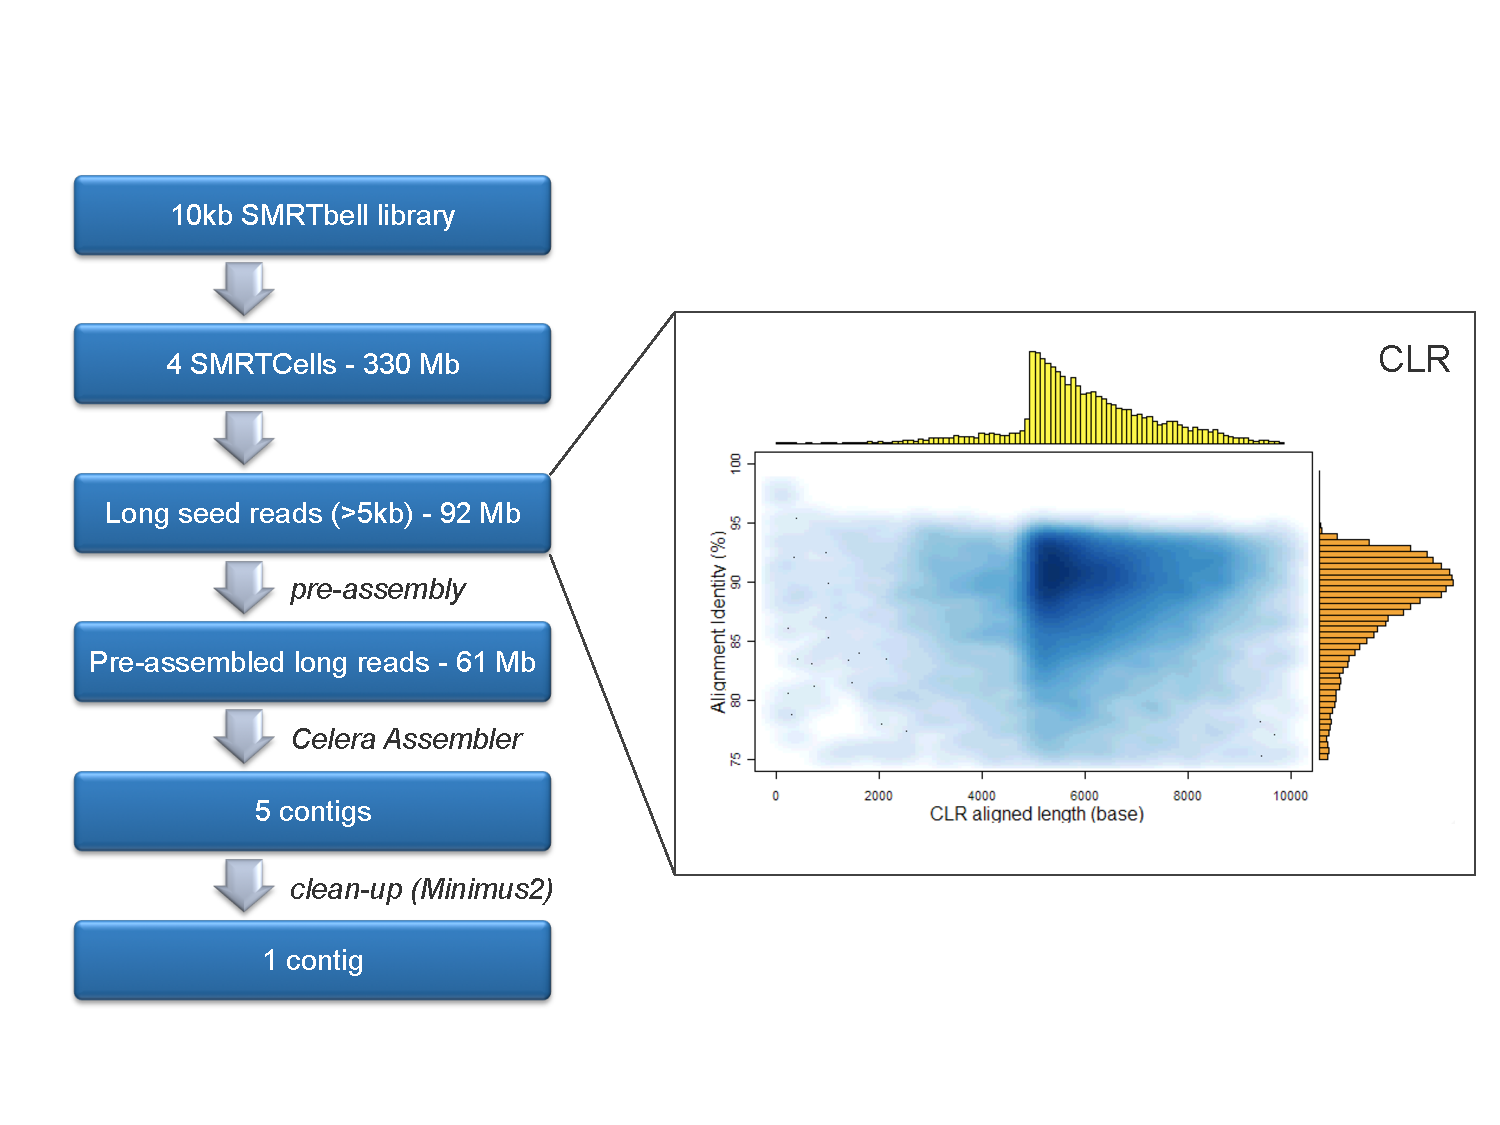
\includegraphics[width=4.75in]{img/hgap-mruber1.pdf}
   \hspace*{0.4in}
\newline \tiny [Slide: Jonas Korlach]
\end{frame}
\begin{frame}
\frametitle{HGAP application: \emph{Meiothermus ruber} (JGI/DOE)}
\label{sec-5-3}

   \hspace*{-0.2in}
   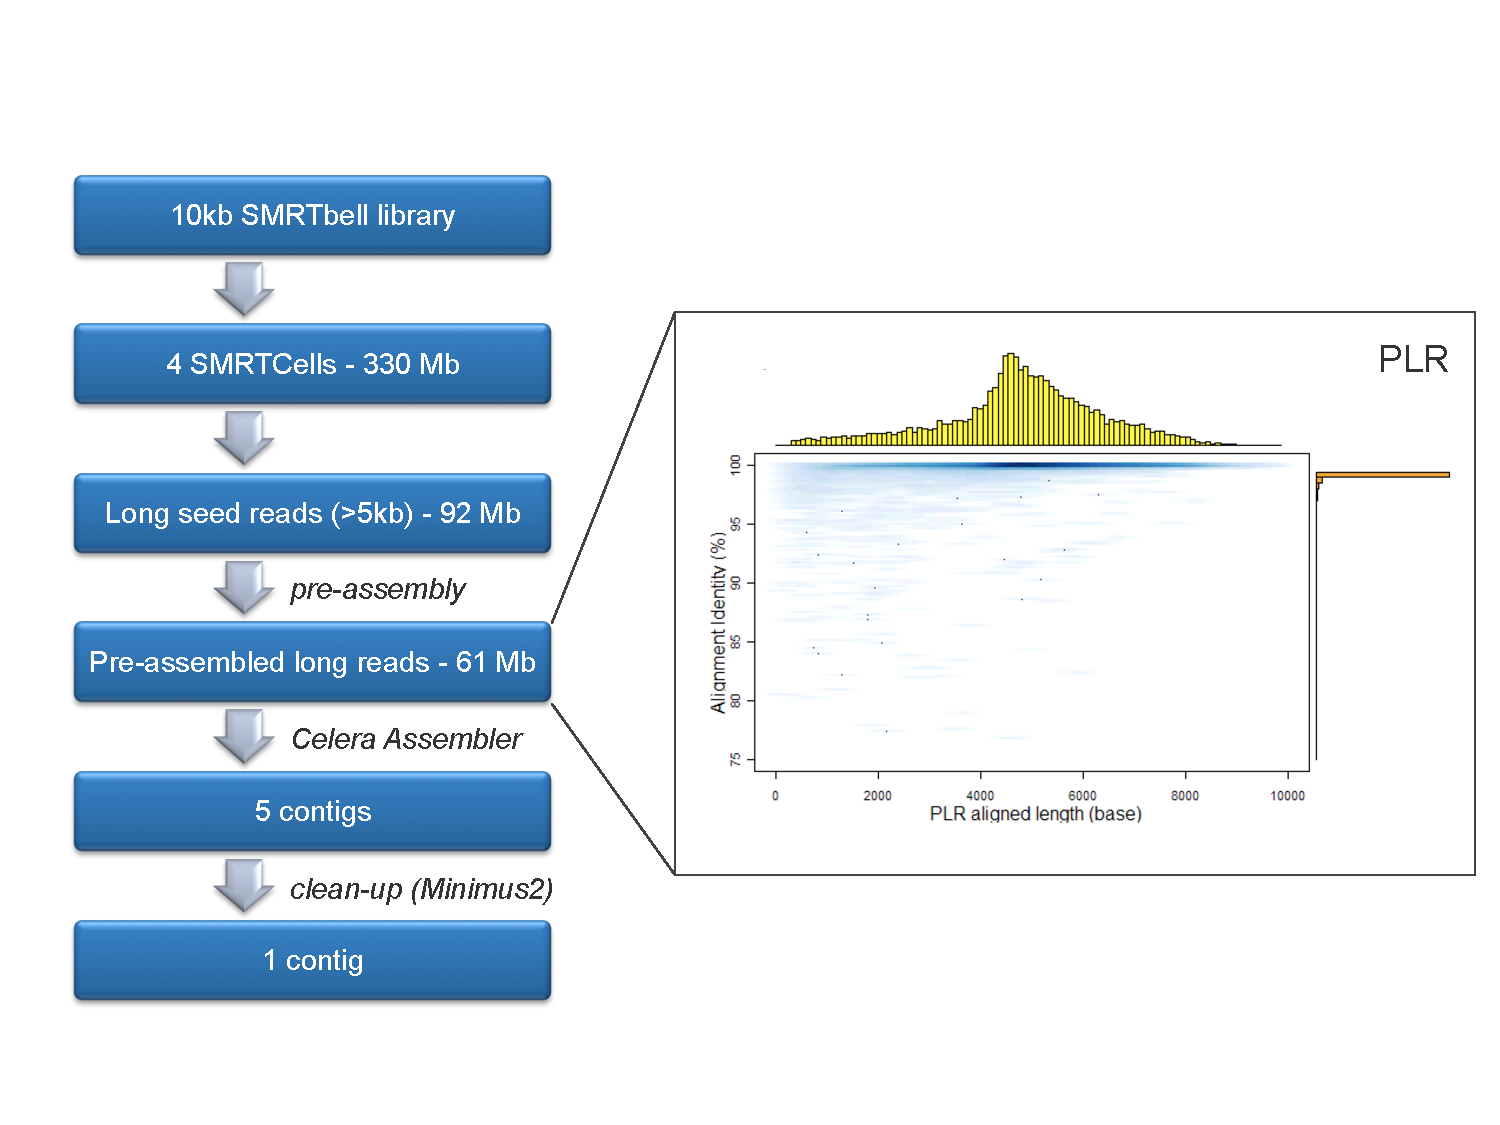
\includegraphics[width=4.75in]{img/hgap-mruber2.pdf}
   \hspace*{0.4in}
\newline \tiny [Slide: Jonas Korlach]
\end{frame}
\begin{frame}
\frametitle{HGAP application: \emph{Meiothermus ruber} (JGI/DOE)}
\label{sec-5-4}

   \hspace*{-0.2in}
   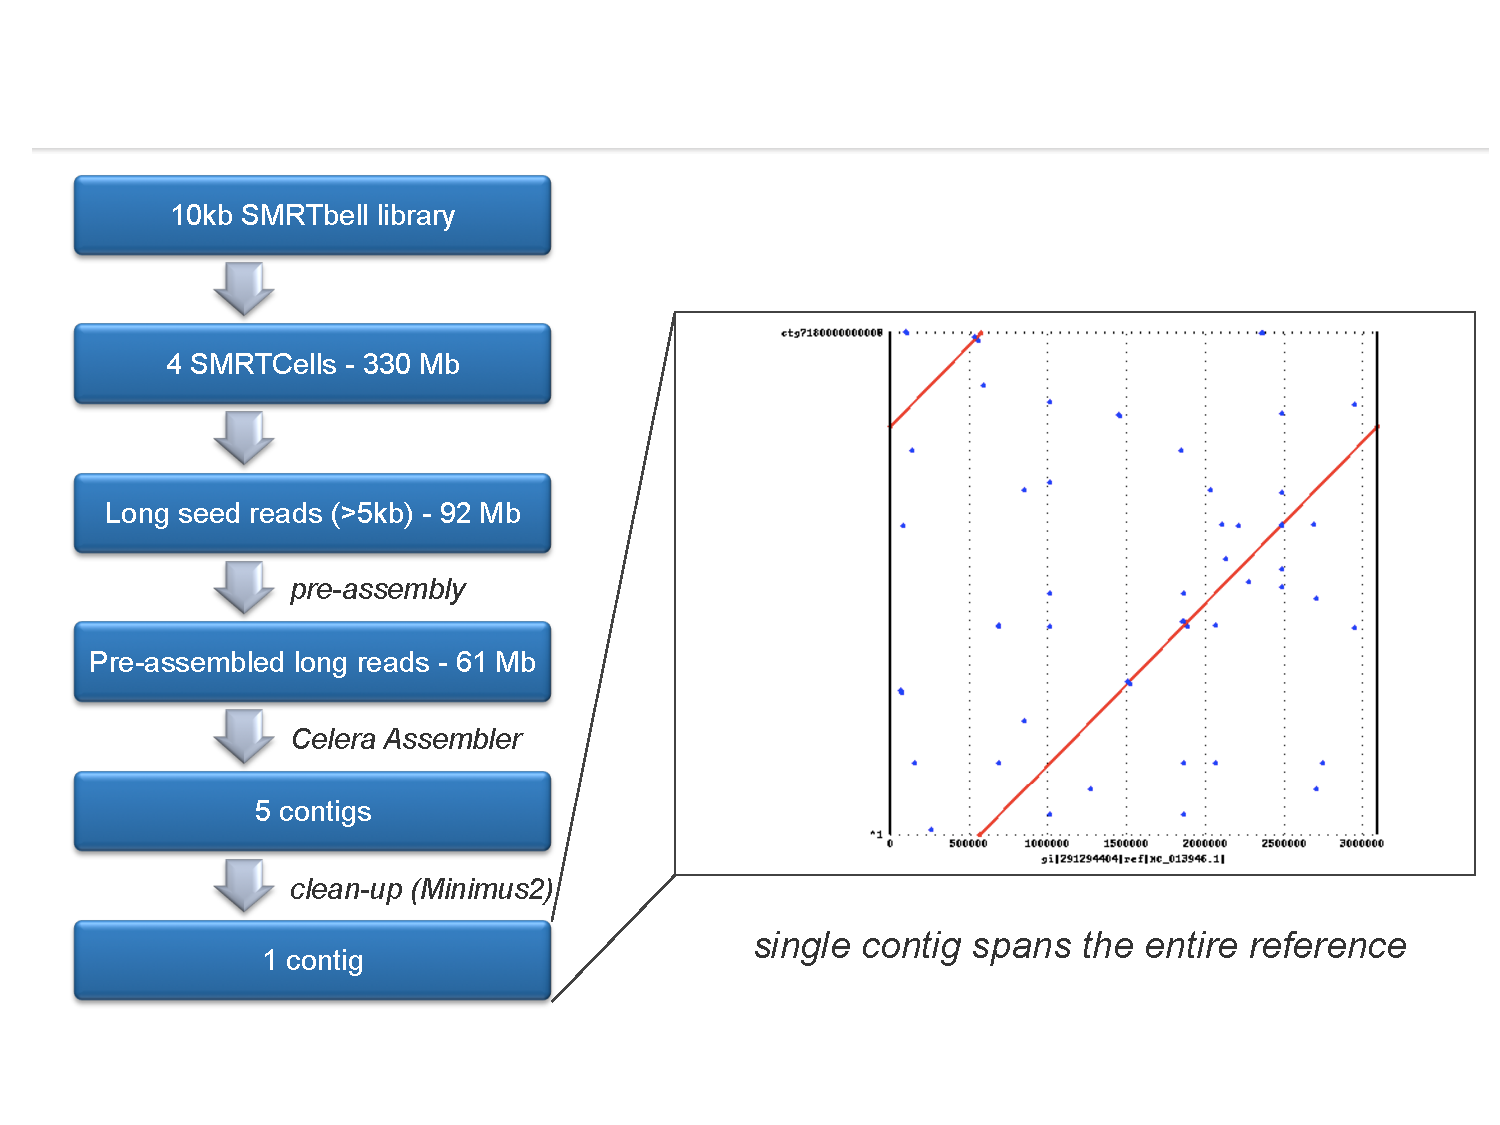
\includegraphics[width=4.75in]{img/hgap-mruber3.pdf}
   \newline \tiny [Slide: Jonas Korlach]
\end{frame}
\section{High accuracy consensus: the Quiver algorithm}
\label{sec-6}
\begin{frame}

  \sectionpage
\end{frame}
\begin{frame}
\frametitle{The consensus problem}
\label{sec-6-1}

\begin{itemize}
\item \emph{Given}: A sequence of reads $\mathbf{R} = \{R^1, R^2, \ldots
    R^{K}\}$ (encompassing basecalls \emph{and} pulse metric features)
\item \emph{Desired}: A consensus sequence $\widehat{T}$ that is, in some sense,
    a ``best'' estimate of the underlying true template sequence $T$ that
    was present in the ZMW.
\end{itemize}
\begin{block}{Applications:}
\label{sec-6-1-1}

    Variant calling, finishing assemblies, circular
    consensus sequencing\ldots{}
\end{block}
\end{frame}
\begin{frame}[fragile]
\frametitle{Example}
\label{sec-6-2}



\begin{center}
\begin{tabular}{ll}
 Template  &  \verb~GATTACA~   \\
\hline
 Read 1    &  \verb~GATTCA~    \\
 Read 2    &  \verb~GATTTACA~  \\
 Read 3    &  \verb~GATACA~    \\
\end{tabular}
\end{center}
\end{frame}
\begin{frame}[fragile]
\frametitle{Multiple-alignment consensus approach}
\label{sec-6-3}

   Do an MSA and let each column vote.


\begin{center}
\begin{tabular}{ll}
 Read 1     &  \verb$GA-TT-CA$  \\
 Read 2     &  \verb$GATTTACA$  \\
 Read 3     &  \verb$GA--TACA$  \\
\hline
 Plurality  &  \verb$GA-TTACA$  \\
\end{tabular}
\end{center}



   Problems:
\begin{itemize}
\item No notion of template vs observations--no clean way to represent our error model.
\item No way to take advantage of QV information
\end{itemize}
\end{frame}
\begin{frame}
\frametitle{Quiver: a model-based approach}
\label{sec-6-4}

\begin{itemize}
\item Encode our sequencing error model as $\Pr(\mathbf{R} \mid T)$
\begin{itemize}
\item Dynamic programming model that can be formalized as a \emph{pair HMM}
       (actually a \emph{pair CRF}).
\end{itemize}
\item Use a greedy algorithm to maximize the likelihood
     $\Pr(\mathbf{R} \mid T)$ in the unknown template $T$.
\end{itemize}
\end{frame}
\begin{frame}
\frametitle{Quiver algorithm overview}
\label{sec-6-5}

   $\mathsf{QuiverConsensus}$ for reference window $W$: (\emph{Rough sketch})
\begin{itemize}
\item Use reference alignment to identify reads $\mathbf{R}=\{R^1, R^2, \ldots R^K\}$
     corresponding to $W$
\item \emph{Throw away reference---not used in computing consensus}
\item $\widehat{T} \leftarrow \mathsf{PoaConsensus}(\mathbf{R})$
\item Repeat until convergence:
     $$\widehat{T} \leftarrow \hat{T} +
     \big\{\text{single base mutations } \mu \, \mid
     \Pr(\mathbf{R} \mid \widehat{T} + \mu) > \Pr(\mathbf{R} \mid \widehat{T}) \big\}$$
\end{itemize}
\end{frame}
\begin{frame}
\frametitle{How to compute $\Pr(\mathbf{R} \mid T)$?}
\label{sec-6-6}


\begin{enumerate}
\item Reads are assumed independent, so
      $$\Pr(\mathbf{R} \mid T) = \prod_{k=1}^{K}\Pr(R^k \mid T)$$
\item For PacBio, indels are the rule, so consider the
      possible \emph{alignments}---the ways $T$ can be construed to
      have generated $R^k$:

      $$\Pr(R \mid T) = \sum_\mathcal{A} \Pr(R, \mathcal{A} \mid T) $$

      \emph{Computed efficiently using a standard Sum-Product dynamic programming approach.}
\end{enumerate}
\end{frame}
\begin{frame}
\frametitle{Sketch of dynamic programming}
\label{sec-6-7}

\begin{itemize}
\item Sum-Product definition:
     \begin{align*}
     A_{ij} \doteq&
     \text{ marginal prob. of an alignment of $R_{0..(i+1)}$ to $T_{0..(j+1)}$ } \\
     B_{ij} \doteq&
     \text{ marginal prob. of an alignment of $R_{i..I}$ to $T_{j..J}$ }
     \end{align*}
\item Sum-Product recursion:
     \begin{align*}
     A_{ij} &= \sum_{m: (i',j') \to (i, j)}   (A_{i'j'} \times \mathrm{moveScore}(m)) \\
     B_{ij} &= \sum_{m: (i, j)  \to (i', j')} (\mathrm{moveScore}(m) \times B_{i'j'})
     \end{align*}
\item For Viterbi approximation, replace \emph{marginal} by \emph{maximum}, replace \emph{sum}
     by \emph{max}.
\end{itemize}
\end{frame}
\begin{frame}
\frametitle{Alignment moves}
\label{sec-6-8}

   \begin{figure}
   \centering
   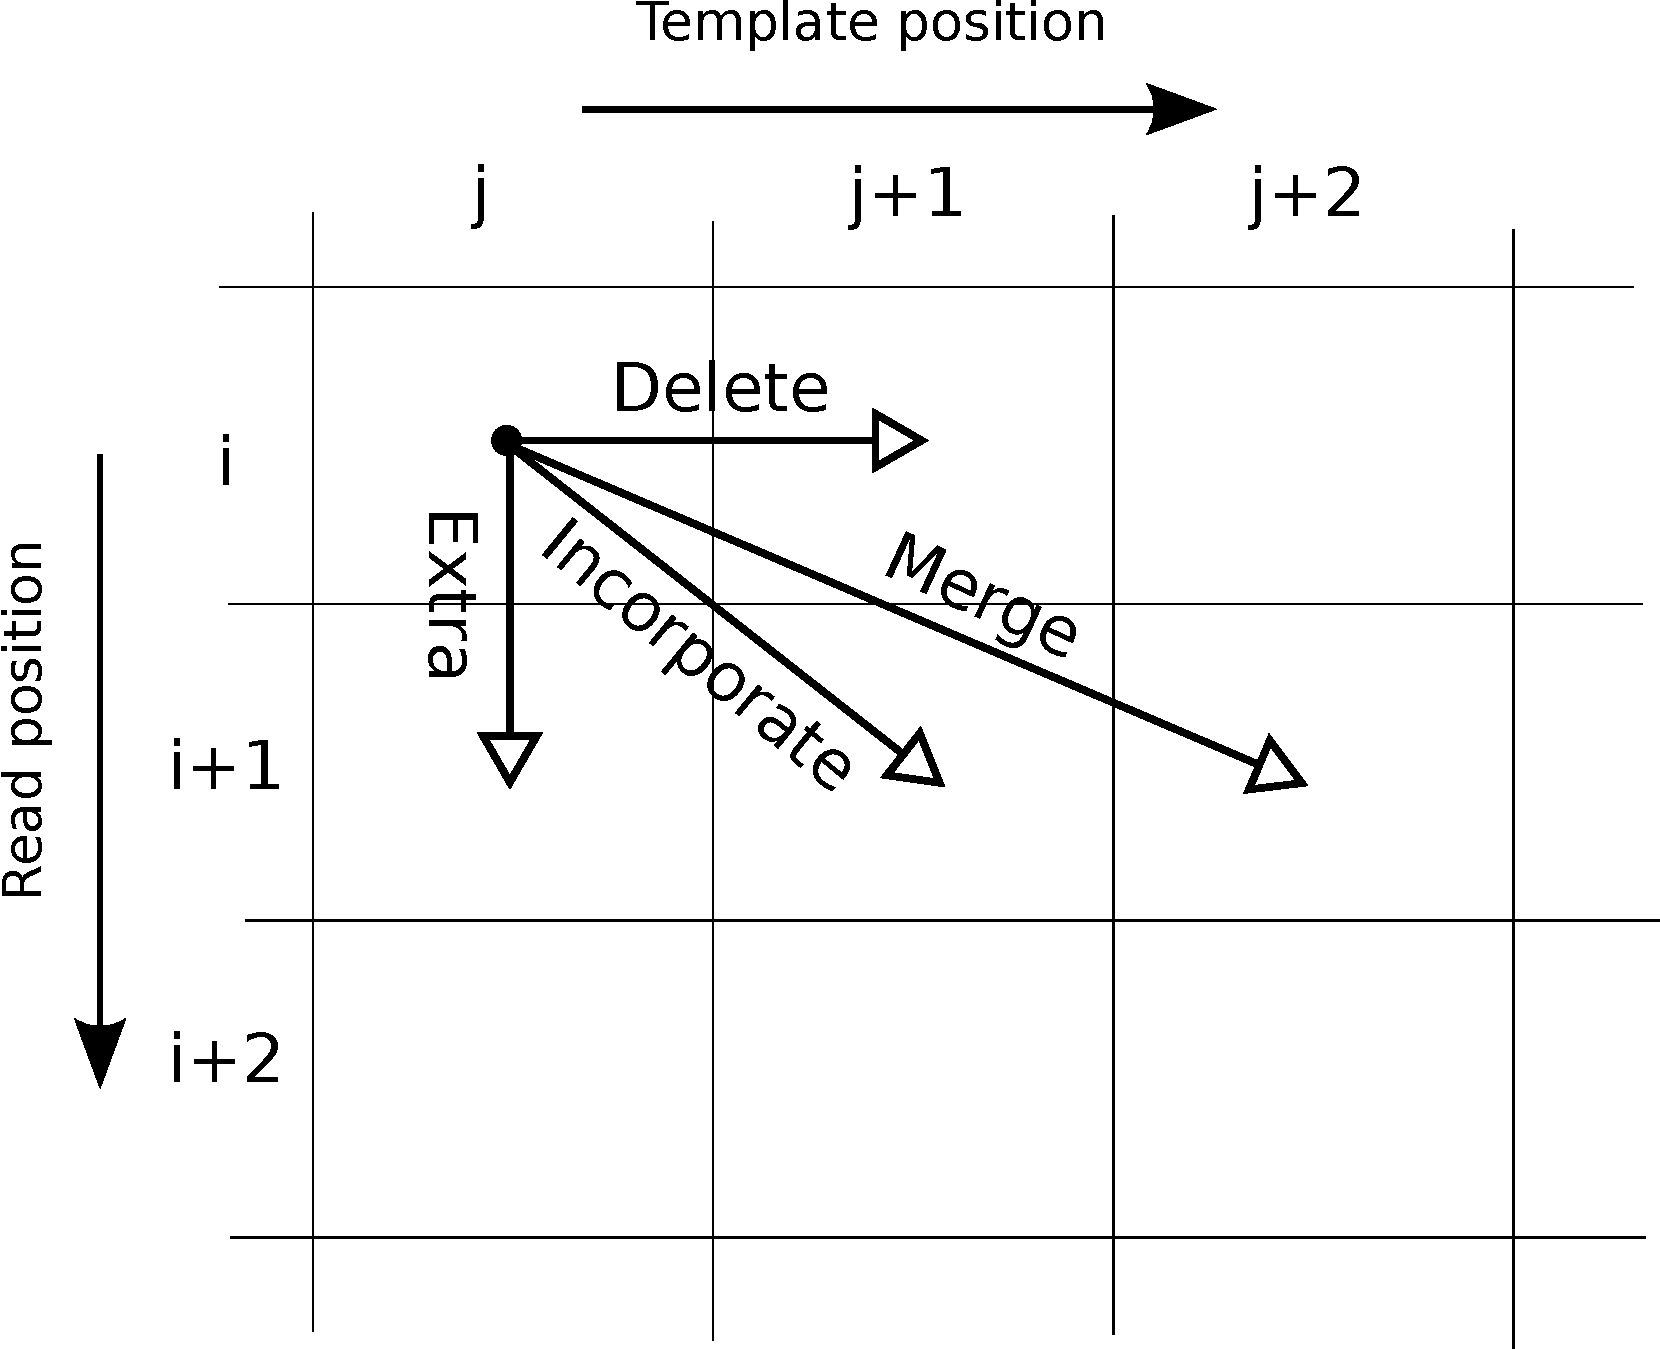
\includegraphics[width=2.5in]{img/moves}
   \end{figure}

\begin{itemize}
\item Additional ``merge'' move helps better account for pulse merging
\item Move scores determined by pulse metrics (QVs)
\end{itemize}
\end{frame}
\begin{frame}
\frametitle{Efficiently computing $\Pr(R \mid T + \mu)$}
\label{sec-6-9}

\begin{itemize}
\item Need to compute score of mutation $\mu$ quickly as this is the
     \emph{rate-limiting operation} in computing the consensus.
\item Do not refill entire $A$, $B$ matrices--we just recalculate two
     columns of $A$ and join with one column of $B$.
\item Exploit forward-backward identity
     \begin{align*}
     \Pr(R \mid T)     =& A_{IJ} = B_{00} \\
                       =& \sum_{m: (i',j') \to (i, j)} A_{i'j'} \times B_{ij},
                       \text{ for \bf{any} $j$}
     \end{align*}
\end{itemize}
\end{frame}
\begin{frame}
\frametitle{Banding for memory and CPU efficiency}
\label{sec-6-10}

   \begin{figure}
   \centering
   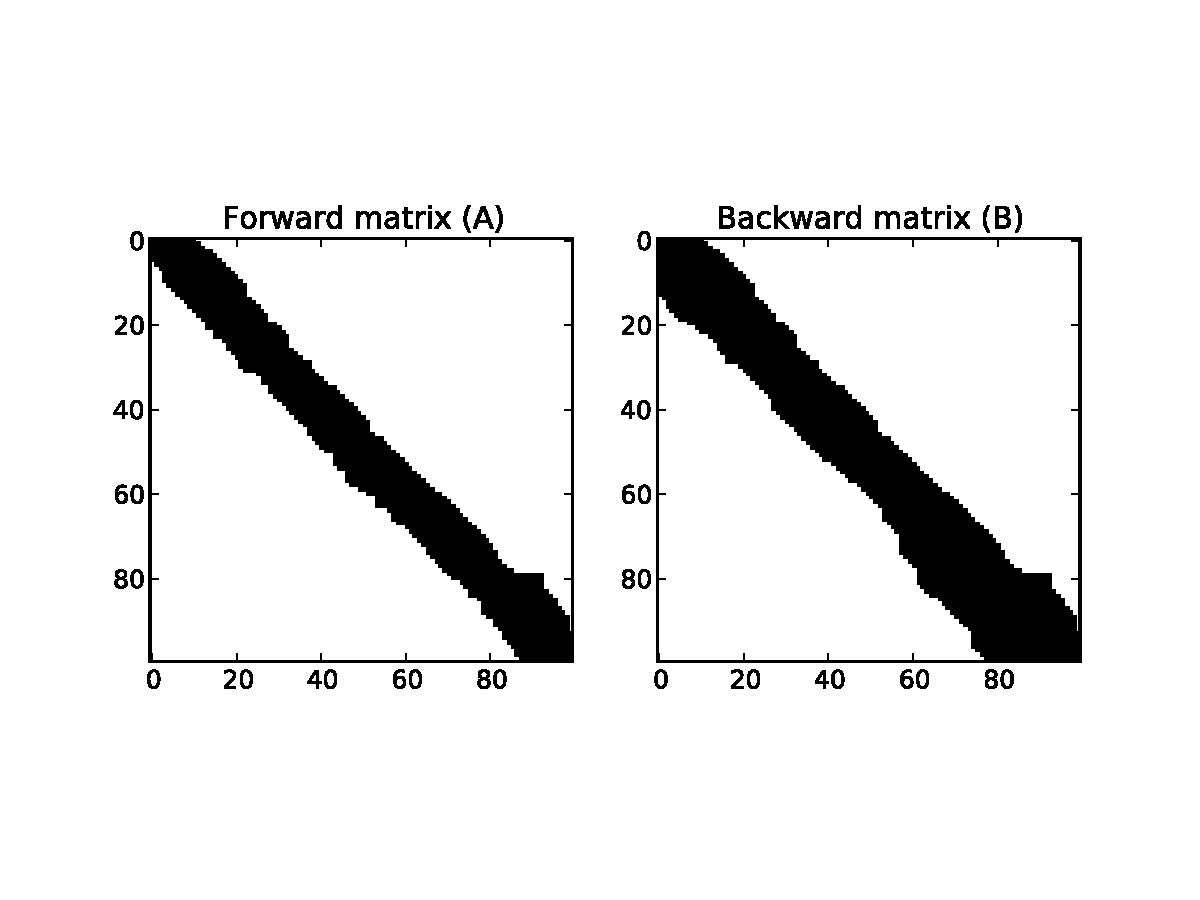
\includegraphics[width=3in]{img/sparsity}
   \end{figure}

\begin{itemize}
\item Optimization 1: \emph{banded dynamic programming}: only compute a narrow band of
     high-scoring rows within each column.
\item Optimization 2: Only \emph{store} the bands.

\begin{center}
\begin{tabular}{lll}
                                  &  Naive     &  Banded    \\
\hline
 Initial computation of $A$, $B$  &  $O(L^3)$  &  $O(L^2)$  \\
 Computation of mutation score    &  $O(L)$    &  $O(1)$    \\
 Storage space for $A$, $B$       &  $O(L^2)$  &  $O(L)$    \\
\end{tabular}
\end{center}


\end{itemize}
\end{frame}
\begin{frame}
\frametitle{Quiver application: polishing \emph{M. ruber}}
\label{sec-6-11}

   Comparison of assembly to Sanger reference:


\begin{center}
\begin{tabular}{lll}
\hline
 Celera assembler ``make-consensus''  &  Q43.4           &  99.9954\%            \\
\hline
 Quiver                               &  \textbf{Q54.5}  &  \textbf{99.99964\%}  \\
\hline
\end{tabular}
\end{center}
\end{frame}
\begin{frame}
\frametitle{Quiver accuracy}
\label{sec-6-12}

   \hspace*{0.2in}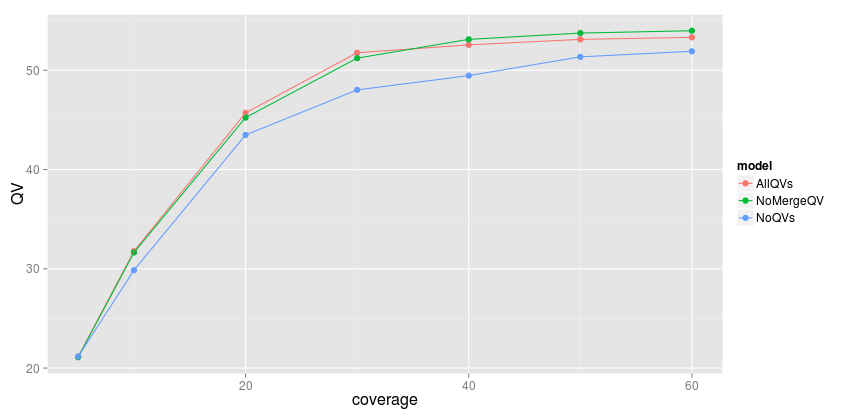
\includegraphics[width=4in]{img/quiver-accuracy-vs-coverage.png}

\begin{itemize}
\item With accuracy > Q50, we are now confronting pesky biological facts!
\begin{itemize}
\item Frequent mutations to our in-house \emph{E. Coli} strain
\item Nonclonal samples
\end{itemize}
\item We are also starting to find errors in Sanger-based references!
\end{itemize}
\end{frame}
\begin{frame}
\frametitle{Quiver extentions}
\label{sec-6-13}

\begin{itemize}
\item Reducing coverage requirements for high accuracy
\item Diploid/polyploid/sample mixtures
\end{itemize}
\end{frame}
\section{Conclusions}
\label{sec-7}
\begin{frame}

   \sectionpage
\end{frame}
\begin{frame}
\frametitle{Conclusions}
\label{sec-7-1}

   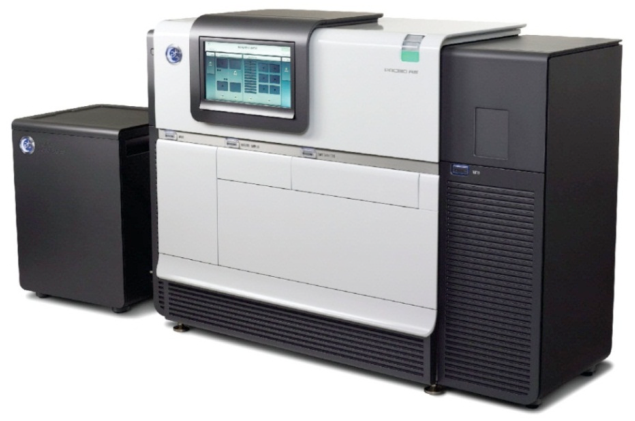
\includegraphics[width=3in]{img/RS.pdf}
   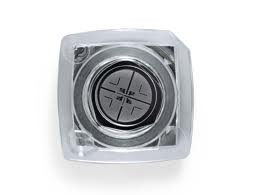
\includegraphics[width=2in]{img/smrtcell.jpeg}

   The PacBio\R \emph{RS} has become a powerful platform for assembly and
   highly accurate sequencing, and is getting better by the week!
\end{frame}
\begin{frame}
\frametitle{Acknowledgements}
\label{sec-7-2}

\begin{itemize}
\item Jonas Korlach
\item Pat Marks (Quiver co-author)
\item Jason Chin
\item Aaron Klammer
\item Collaborators at DOE-JGI, Eichler lab
\end{itemize}
\end{frame}

\end{document}
